\documentclass[11pt]{article}

\usepackage{common}
\usepackage{booktabs}
\usepackage[margin=1in]{geometry}
\usepackage{hyperref}
\title{The Analytics Edge, Final Report:\\ Building an Article Recommender for Bleacher Report Basketball}
\author{for Professor Dimitris Bertsimas and Emma Gibson \text{ } \\ \\ by Stephen Albro \& Cyrille Combettes \\ salbro@mit.edu, cyrille@mit.edu}
\begin{document}
\maketitle{}


\section{Motivation and Project Abstract}
%As avid basketball fans, we have enjoyed reading a variety of NBA articles to keep up-to-date on the league during our busy year in the MBAn program.  Bleacher Report, a primary digital destination for sports article readers, contains well written articles covering the league, and competes as advertisement real-estate with the likes of ESPN.com, FoxSports.com, CBSSports.com, SBNation.com, and others.  In this paper, we develop a prototype for an article recommendation system using state of the art natural language processing techniques for both cleaning and analyzing bleacher report articles.
In an age of cut-throat digital competition, it is vital for websites to be able to retain visitors. Bleacher Report, a primary digital destination for sports article readers, contains well written articles covering the league, and competes as advertisement real-estate with the likes of ESPN.com, FoxSports.com, CBSSports.com, SBNation.com, and others. The hope for a Bleacher Report article reader is two-fold. First, that the visitor jumps from article to article \textit{on the website}, rather than returning to the search engine results page.  Second, that the visitor falls in love with the content and coverage of Bleacher Report's articles, and develops a loyalty to the website. In this paper, we develop a prototype for an article recommendation system using state of the art natural language processing techniques for both cleaning and analyzing bleacher report articles.

We feel that having a micro targeted article recommendation system would provide Bleacher Report with an analytics-based edge over its competitors, since well targeted articles could increase the chances of prolonged visits, and increase website loyalty by making users feel known.   A reasonable document-recommendation strategy embed documents as vectors and then use K Nearest Neighbors to group documents together. Our project focuses on exploring the right article embedding strategy.  At first, we ran an experiment to find the most promising from among  three primary methods: word2vec, Non-negative Matrix Factorization (NMF), and Latent Dirichlet Allocation (LDA).  We evaluated each approach using a hand-crafted test set.  A preliminary analysis revealed LDA to be the most promising strategy, and so we focused the rest of our efforts on developing a quality LDA topic model, which we then used to produce visualizations of the topic landscape of Bleacher Report's NBA articles. 

\section{Data Collection}
Bleacher Report does not provide easy access to their articles in a public database.  However, News API is a company that provides API access to major news articles from a variety of sources, including Bleacher Report.  Using NewsAPI, we queried Bleacher Report NBA articles from October 17, the start of the 2017-2018 NBA season. Our entire query consisted of joining words like basketball and NBA with all 30 teams and the top 25 active players.  In the end, we received 3314 URLs (with their corresponding authors, titles, and other metadata) in return.  We then wrote a script to request the webpage for each URL and scrape its content, picking the paragraphs out of the HTML.

\section{Data Cleaning}
In the real world, data is never clean, and this is magnified in the case of textual data. There were a number of preprocessing steps we had to do before our articles were ready for analysis. In our cleaning efforts, we made decisions \textit{based on the purpose of our task} - to cluster documents for better recommendation power.  In particular, a bag-of-words approach to cleaning was preferred over one that preserved punctuation and grammar. 

%\subsubsection{Punctuation Removal, Initial Stopwords, and Lowercasing}
First, we tokenized each article. In natural language processing, tokenizing is a way of chopping up a document into pieces, the most obvious way being to tokenize by \textit{word}, which is what we initially did.  Next we discarded any non-alphabetical tokens (e.g. 8pm, 704, !, .), and converted every token to lower case.  After converting everything to lower case, we did our first round of stop word removal (we remove more later).  In  NLP a stop word is any word that you remove because its insignificant for your application. In this first round, we removed basic articles (the, a) and about 170 other words deemed insignificant by Python's Natural Language Toolkit, mostly personal pronouns and simple verbs.

%\subsubsection{Specialized NBA Tokenization}
Next, since we were analyzing NBA articles, we had to take into account the fact that each player (and each team for that matter) can be referred to in a variety of ways. For example, the NBA superstar LeBron James can be called LeBron James, LeBron, Bron, or James, and the Boston Celtics might be formally referred to as such in the title, but in the article's body they might just be Boston. For this reason, we compiled lists of team names, players, and coaches.  For each article, we replaced all forms of each entity with its underscored full version, so that for example LeBron James would always be lebron\_james, no matter if he occurred as Bron, James, or Lebron in a given sentence.  At times it was necessary to infer from ambiguous usage. We concluded that, for example, the word \textit{Boston} should be replaced by boston\_celtics only if the entire phrase Boston Celtics appeared somewhere in the article.  This specialized, application-specific tokenization step allowed us to capture much more information about each superstar/team/coach than would for example, treating Bron as a separate player as Lebron.

%\subsubsection{Stemming Each Word}
Next, we needed to address the fact that sometimes the same words take different forms. A reasonable assumption that we made the words playing, played, play, and plays all capture the same information as far as topic modeling goes. Thus we decided to \textit{stem} each word, which in NLP means to convert every word into its root form.  Python's Natural Language Toolkit provides a stemmer.

%\subsubsection{Trimming Down the Vocabulary}
A model is only as good as its input, and so as a last step, we realized that we needed to trim down the vocabulary of our articles. In NLP, a \textit{vocabulary} is simply the complete set of words that the model knows about.  We already removed basic stop words, but figured that many more could be removed. For clustering documents, its important to identify information-containing words (player and team names, high-impact verbs, league terminology), and less important to identify mundane nouns and verbs (table, cup, gave, took) even if their not considered stop words.

To identify our functional vocabulary, we used a \textit{document frequency} approach. The document frequency of a given word is simply the fraction of documents (in this case articles) that the word appears in. The word \textit{the}, for example, has a document frequency of 1.0. If a word occurs too \textit{infrequently}, it is probably a unique name or an article-specific entity, and thus unhelpful in forming clusters. On the other hand, if a word occurs too \textit{frequently}, it is probably a common word and thus contains very little information related to topics.

Thus, we sought lower and upper document frequency cutoffs for including a word in the vocabulary.  As a sanity check, we knew our upper cutoff had to be at least high than the document frequency of LeBron James (0.22, he the most famous superstar), since every player should be in our vocabulary. After seeing irrelevant words present with an upper cutoff of even 0.5, we knew that the upper cutoff had to be lower than that, and decided upon 0.23 after experimentation (at this point the eye test was possible). Our lower cutoff was 0.01, which means that if a word appeared in less than 34 out of 3314 total articles, it was discarded.  In total, the new vocabulary consisted of about 3500 tokens with document frequencies within the range (0.01, 0.23), including the major players and teams, and, we think, the important, topic-filled sports and NBA terminology. To give a sense, some of the first few (stemmed) tokens printed from our vocab set include \textit{fewest, monday, march, eric\_bledso, toronto, decid, blowout, jae\_crowd,} and \textit{aggress}.  

%Jae Crowder and Eric Bledso are included, as are all NBA players by virtue of Lebron James being included.
\section{Topic Modeling with Latent Dirichlet Allocation}
In order to cluster articles for recommendation, it is necessary to embed them in some vector space.  There are many ways to approach this problem.  For this, project we wanted to dive deep into one model rather than shallow into several.  Therefore, we ran an initial experiment on three approaches to find the most promising.  LDA turned out to be the most promising and the most exciting, so we leave that to be discussed in the following section.  Other than LDA, the two article-embedding approaches we tried involved a word2vec model, and Non-Negative Matrix Factorizatoin (NMF).  In the appendix we briefly discuss them, as well as our intial experiment to find the most promising model.

We spent the rest of our project diving more deeply into finding a quality LDA model, and using that to explore the landscape of topics for Bleacher Report NBA articles. 

\subsection{Topic Modeling and LDA Background}
In the following section, define \\
$D = \{d_1, d_2, ... d_N \}, \quad$ the set of $N$ documents (articles) obtained from Bleacher Report \\
$V = \{w_1, w_2, ... w_M \}, \quad$ the set of $M$ words in the final vocabulary \\
$T = \{t_1, t_2, ..., t_K\}, \quad$ the set of $K$ topics in the documents 

The first way we approached the question of document similarity was topic modeling.  In topic modeling, we attempt to infer which \textit{topics} are present among the documents, and then after that, to identify which topics belong to each particular document, and in what proportion.  Here a \textit{topic} is simply a probability distribution over the words in the vocabulary.  For each topic, each word has a probability of being chosen.  The task is difficult, because we are trying \textit{both} to infer the topics themselves (all we provide in advance is $K$, the number of topics), \textit{as well as} the topic-composition of each document.

We decided upon a specific Topic Model known as Latent Dirichlet Allocation (LDA).  LDA assumes that documents are created according to the following generate process: \\
$\text{} \quad$ 1. Randomly generate a distribution over topics\footnote{This requires a distribution over a distribution. The  topic distribution is assumed to have a Dirichlet prior, giving the model its name}. \\
$\text{} \quad$ 2. To come up with each word in the document: \\
$\text{} \quad$ $\quad$ a. Randomly choose a topic. \\
$\text{} \quad$ $\quad$ b. Randomly choose a word from that topic. 

The main task of LDA is then to infer two parameters by maximizing the likelihood of the articles observed according to that process: \\
$\text{} \quad \beta_t$: the distribution over words for topic $t$: $\mathcal{P}(w | t) \quad \forall w \in V$ \\
$\text{} \quad \theta_{dt}$: the proportion of document $d$ that came from topic $t$: $\mathcal{P}(t | d) \quad \forall t \in T$ 

%LDA infers these parameters according to which values maximize the likelihood of the data observed.
These estimates allow us to express each document as a vector, which is a distribution over the topics it contains.  The vectorized documents can then be clustered based on their topical composition. The idea is that if I love the topic of statistics and I also love the topic of Lebron James, I will be recommended articles about Lebron James' statistics. 
%LDA is considered a bag-of-words model because the generative story says nothing about grammar. For topic modeling, we do not care about grammar anyway.    

\subsection{Training LDA with Grid Search}
We trained LDA models on the cleaned Bleacher Report articles using Python's sklearn libraries.  When training the models, two hyper-parameters needed to be fine-tuned. The first was $K$, the number of topics to ask for.  The second was $\gamma$, the learning rate of the solver.  (TALK MORE ABOUT THIS?). We decided to use a grid search cross validation approach. Since topic modeling is an unsupervised problem, there was no need for a separate validation set.  Instead we used the log-likelihood of the trained model as our measure of model quality. 

First, we searched $k \in \{10, 15, 20, 25, 30\}$ and $\gamma \in \{.5, .7, .9\}$. On the left is a chart of the grid search results, the log likelihoods for each parameter duo. After discovering that the best hyper-parameters were found to be $k=10$, $\gamma = 0.7$, we decided to narrow down the grid search further (right) to find the absolute best number of topics.  After a narrowed grid search over $k \in \{10, 11, 12, 13, 14\}$ and still $\gamma \in \{.5, .7, .9\}$, we moved forward with the optimal $k=13$ topics (and $\gamma = 0.7$). \\

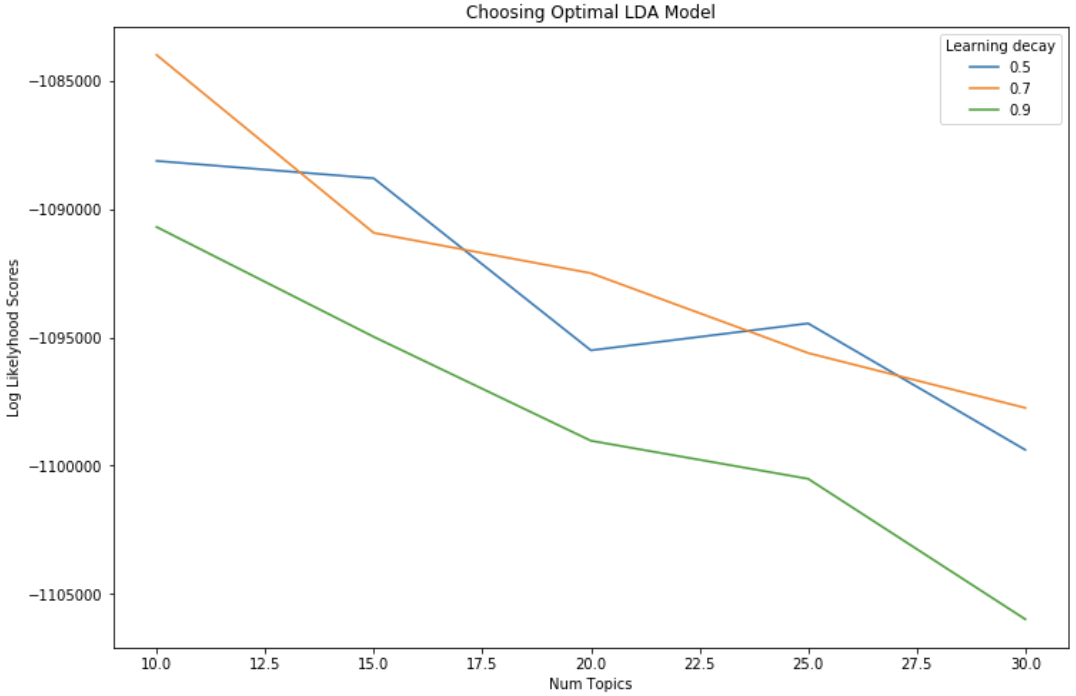
\includegraphics[width=250pt]{gridsearch.png} 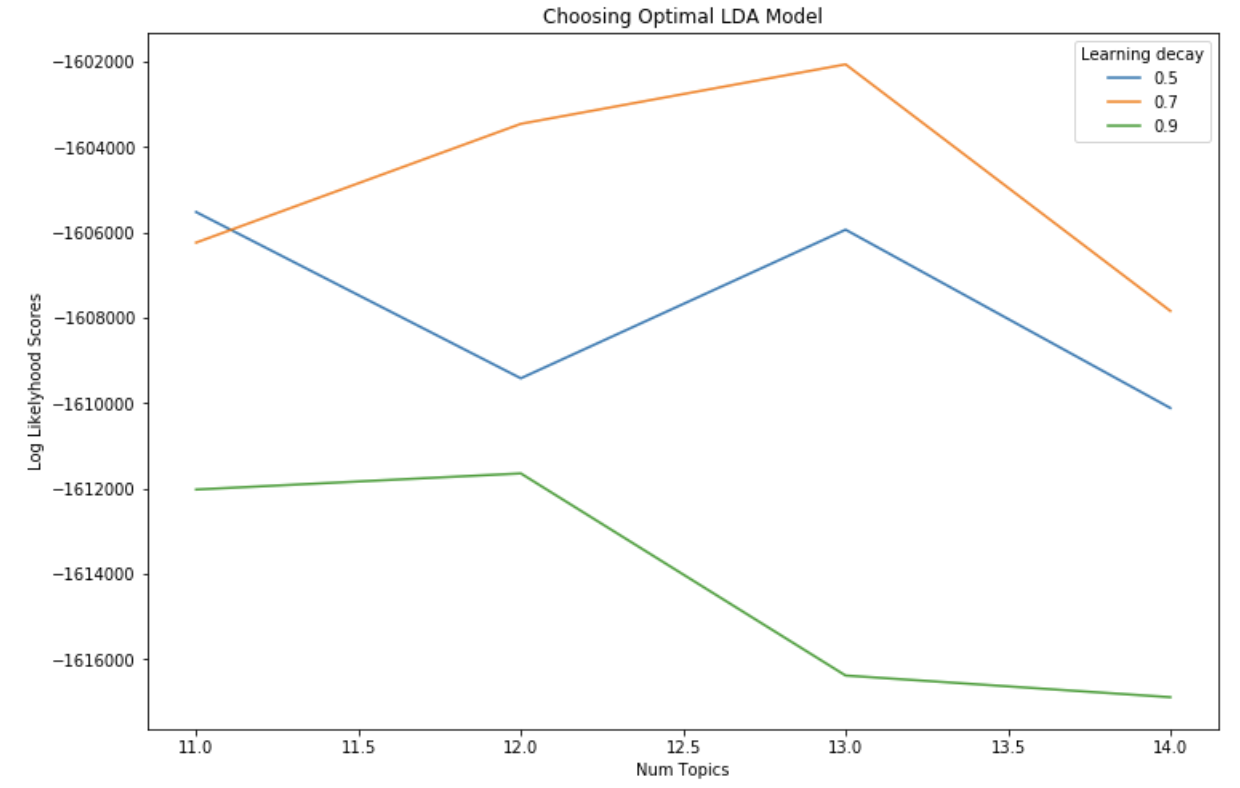
\includegraphics[width=250pt]{gridsearch2.png} 

\subsection{LDA Results and Visualization}
As avid NBA fans, we were very pleased to discover that our topics made great sense.  We visualized them using LDAvis, a method for visualizing LDA topics developed by Carson Siever and Kenneth Shirley \footnote{Sievert, Carson and Shirley, Kenneth. "LDAvis: A method for visualizing and interpreting topics". \textit{Proceedings of the Workshop of Interactive Language Learning, Visualization, and Interfaces}, pages 63-70, Baltimore, Maryland, USA, June 27, 2014. Their Github can be found \href{https://github.com/cpsievert/LDAvis}{here}}.  The visualization has two primary components.  On the left, the blue circles represent the topics. The size of each circle represents the proportion of its topic occurance across all documents. The positions of the circles is meant to be a 2D projection of their locations with respect to each other in the topic space. Specifically, a matrix of inter-topic distances is generated, \footnote{Remember that a topic is a probably distribution over all words in the vocabulary. The distance between two topics is found by computing the Jensen-Shannon diveragence between their distribution.}, where each row in the matrix contains one topic's distances to every other topic.  The $K$-dimensional distance rows are then shown in 2 dimensions using Principal Component Analysis \footnote{Though the topics themselves sense, we cannot detect any semantic meaning in the first two principal components.} This visualization technique is known as \textit{multidimensional scaling}, and typically performed on distance matrices as in this case. 

On the right, the red bars indicate the estimated number of times a given term came from a given topic. When you hover over a topic, the 30 most relevant terms from that topic are shown.\footnote{$\text{relevance}(w | t) = p(w | t) + p(w | t)*p(w)$}  Our visualization is interactive, and we recommend that you run it in our notebook, RUNME.ipynb.  However we we show a few topics here. 

The most prevalent topic, 1, is all about player statistics (steals, blocks, defensive and offensive rates, ranks, percentages, etc.). It makes sense that this is the most prevalent topic in a corpus full of sports articles. 

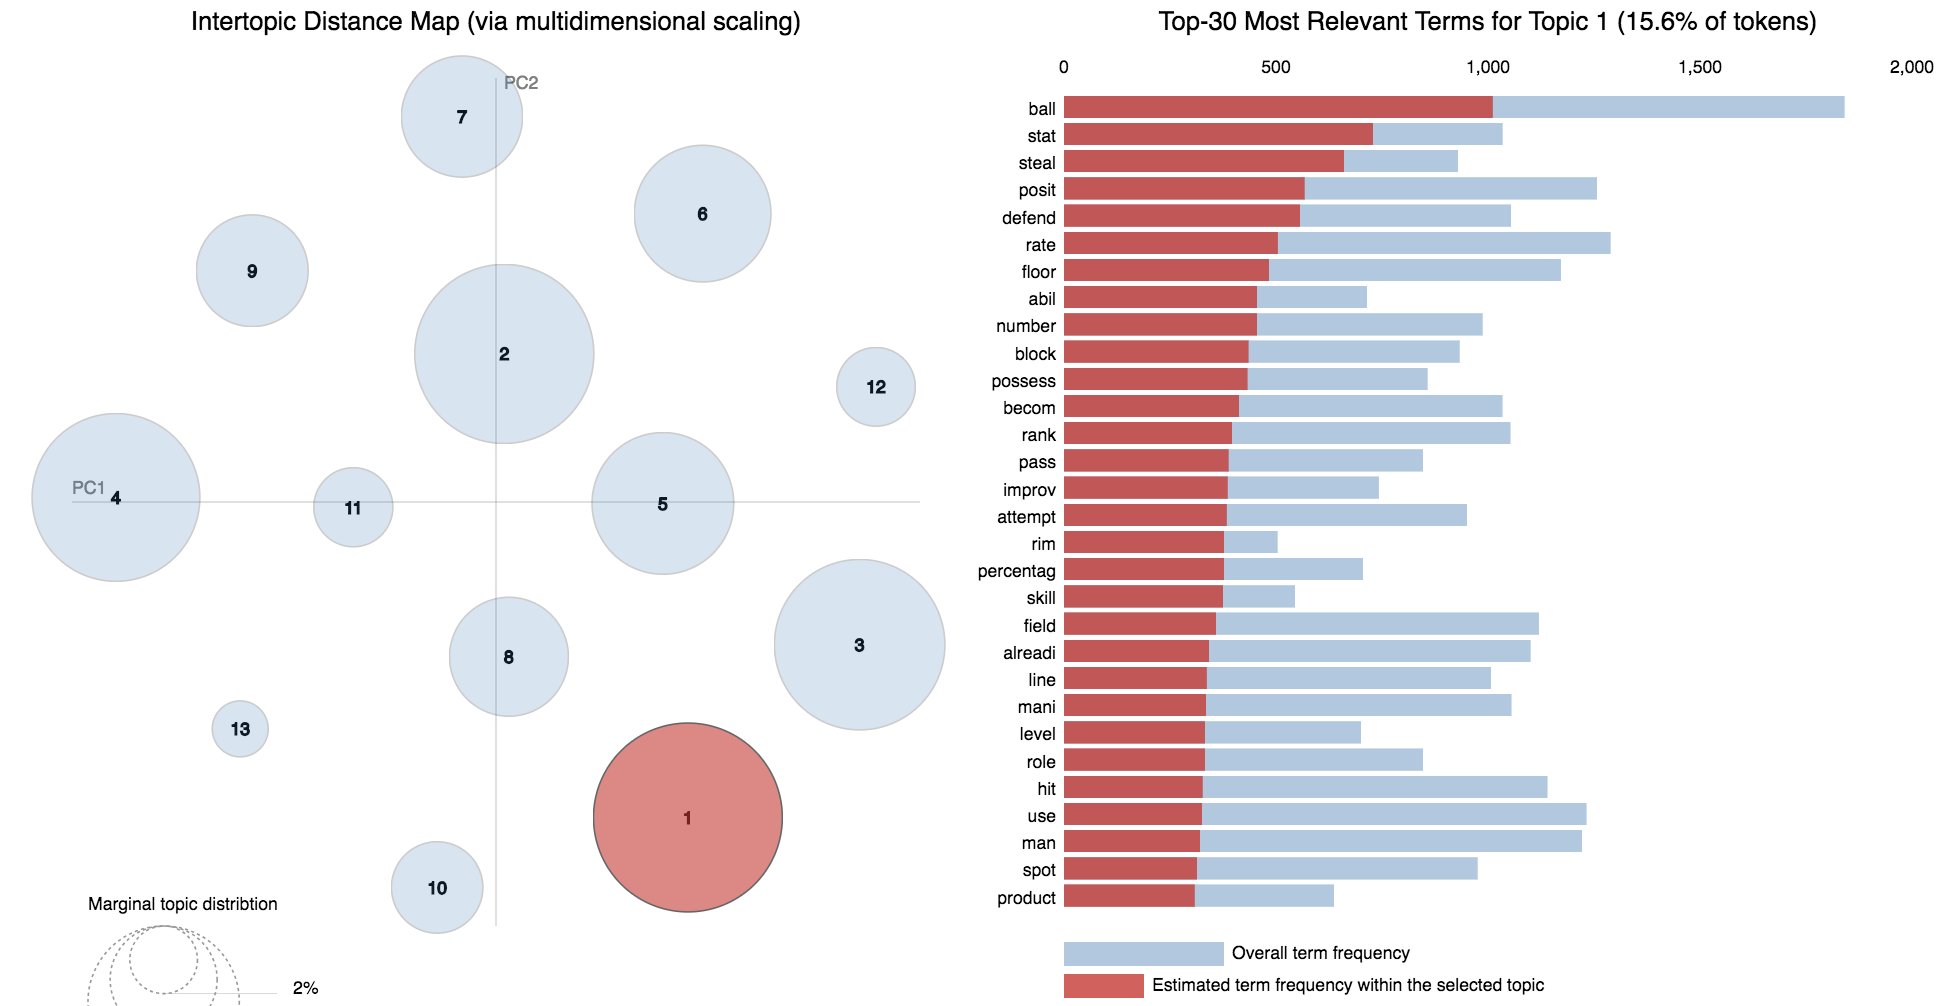
\includegraphics[width=470pt]{1.png} 

To its right, topic 3, seems to be about the Golden State Warriors, the best team in the NBA (mostly because of superstars Stephen Curry and Kevin Durant), and their competition in the Western Conference (including James Harden's Rockets and Russel Westbrook's Thunder). 

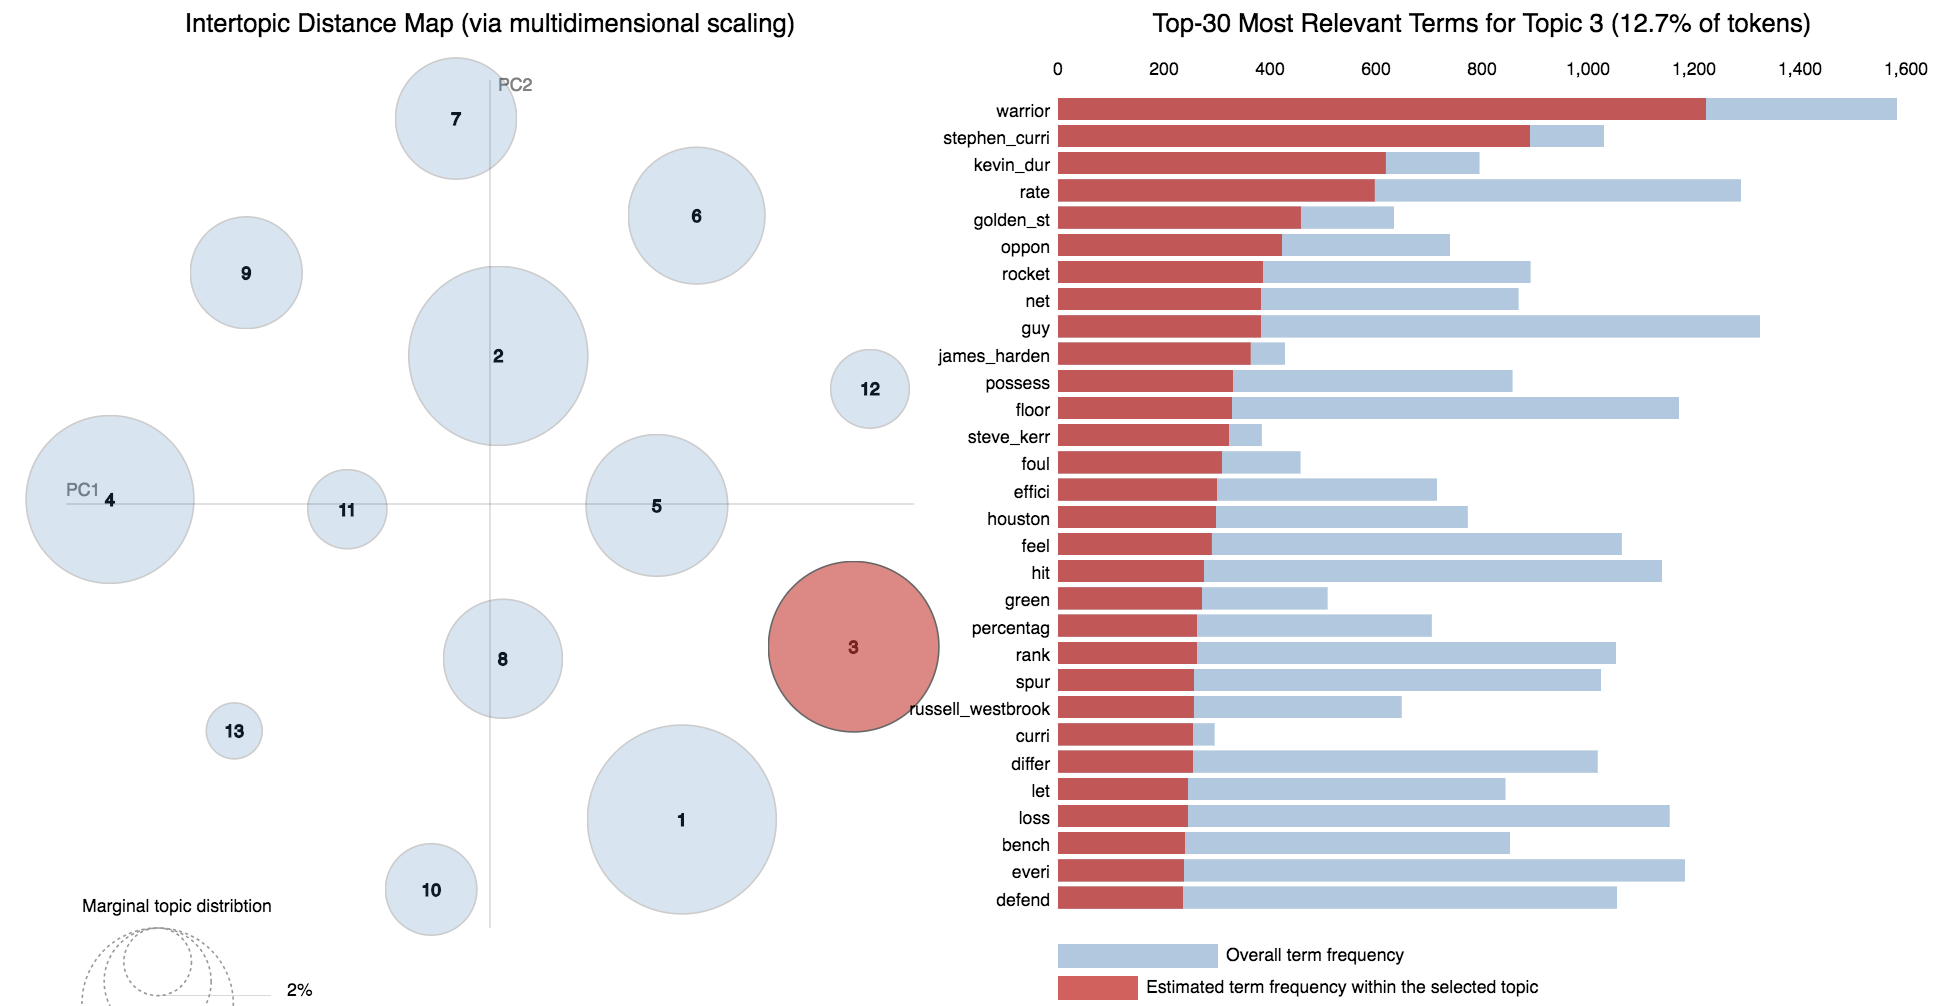
\includegraphics[width=470pt]{3.png} 

Topic 4 is all about the economics of the NBA, including trade deals, free agency signing decisions, and salary information.

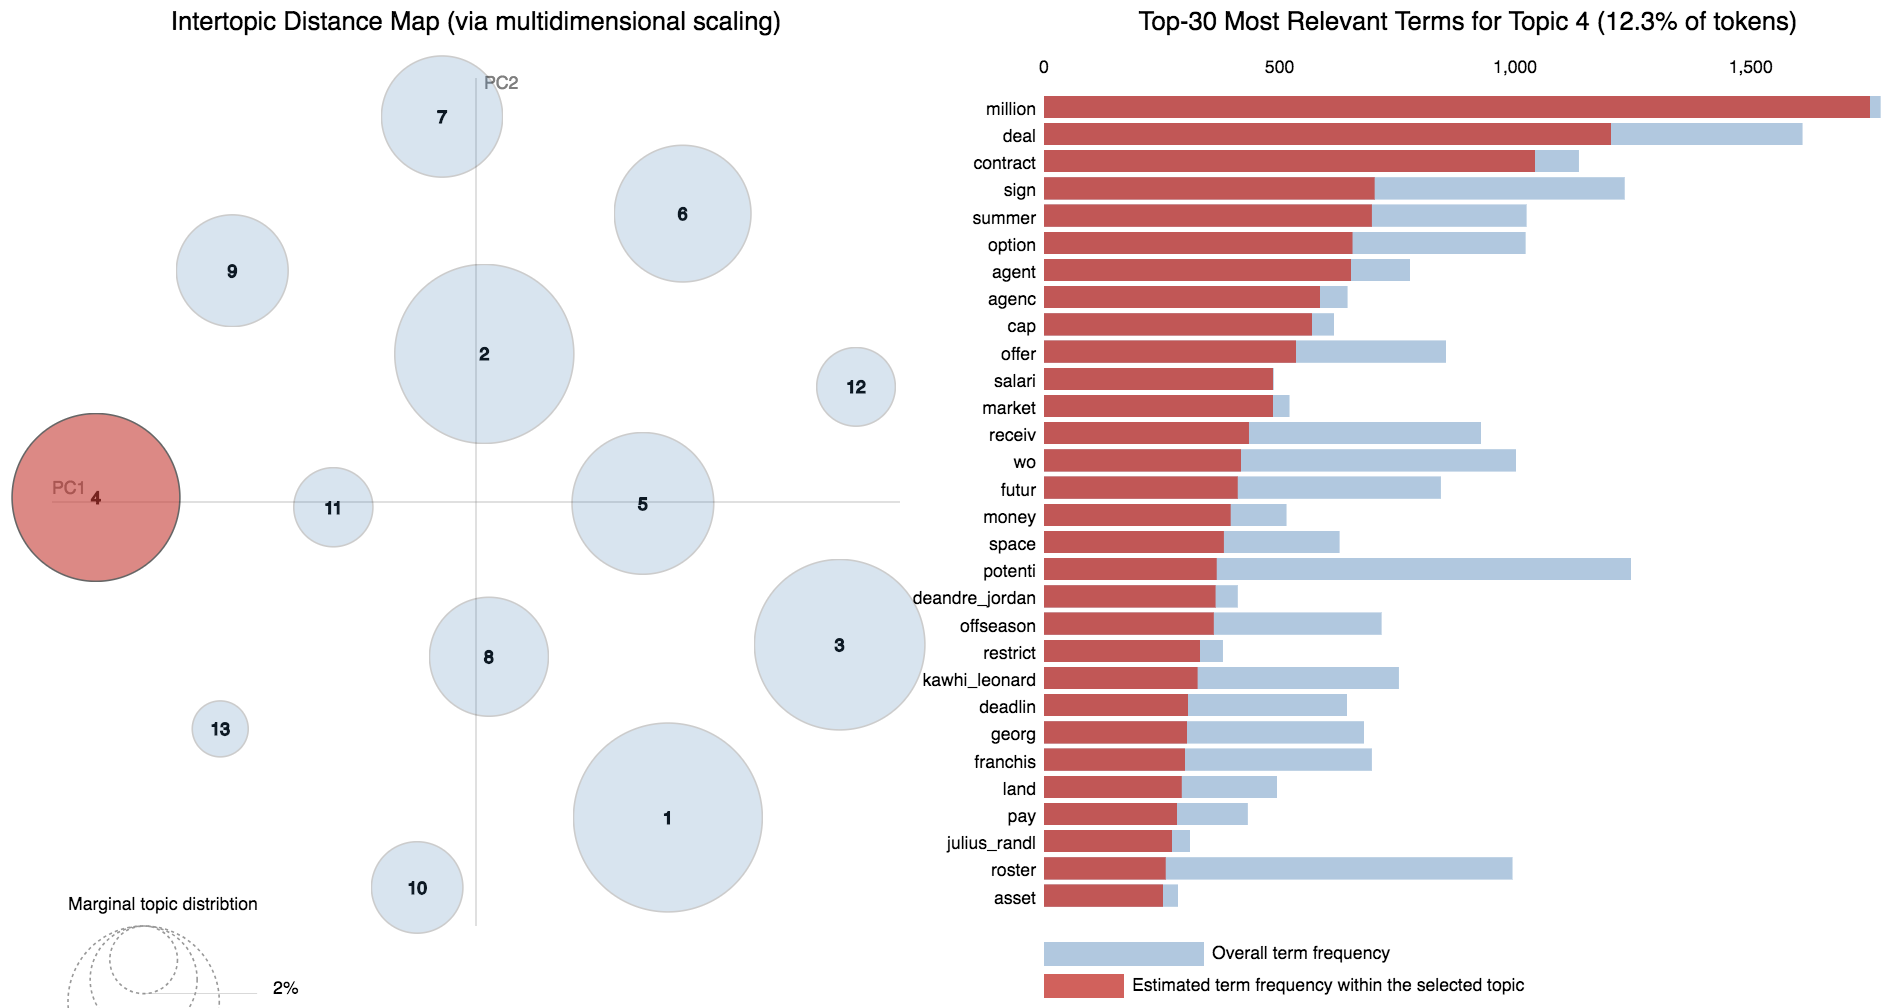
\includegraphics[width=470pt]{4.png} 

Topic 5 is our personal favorite, as it is all about Lebron James.  The most salient words in topic 5 are Lebron, his team mates, his team name, his coaches, and his major rivals.  

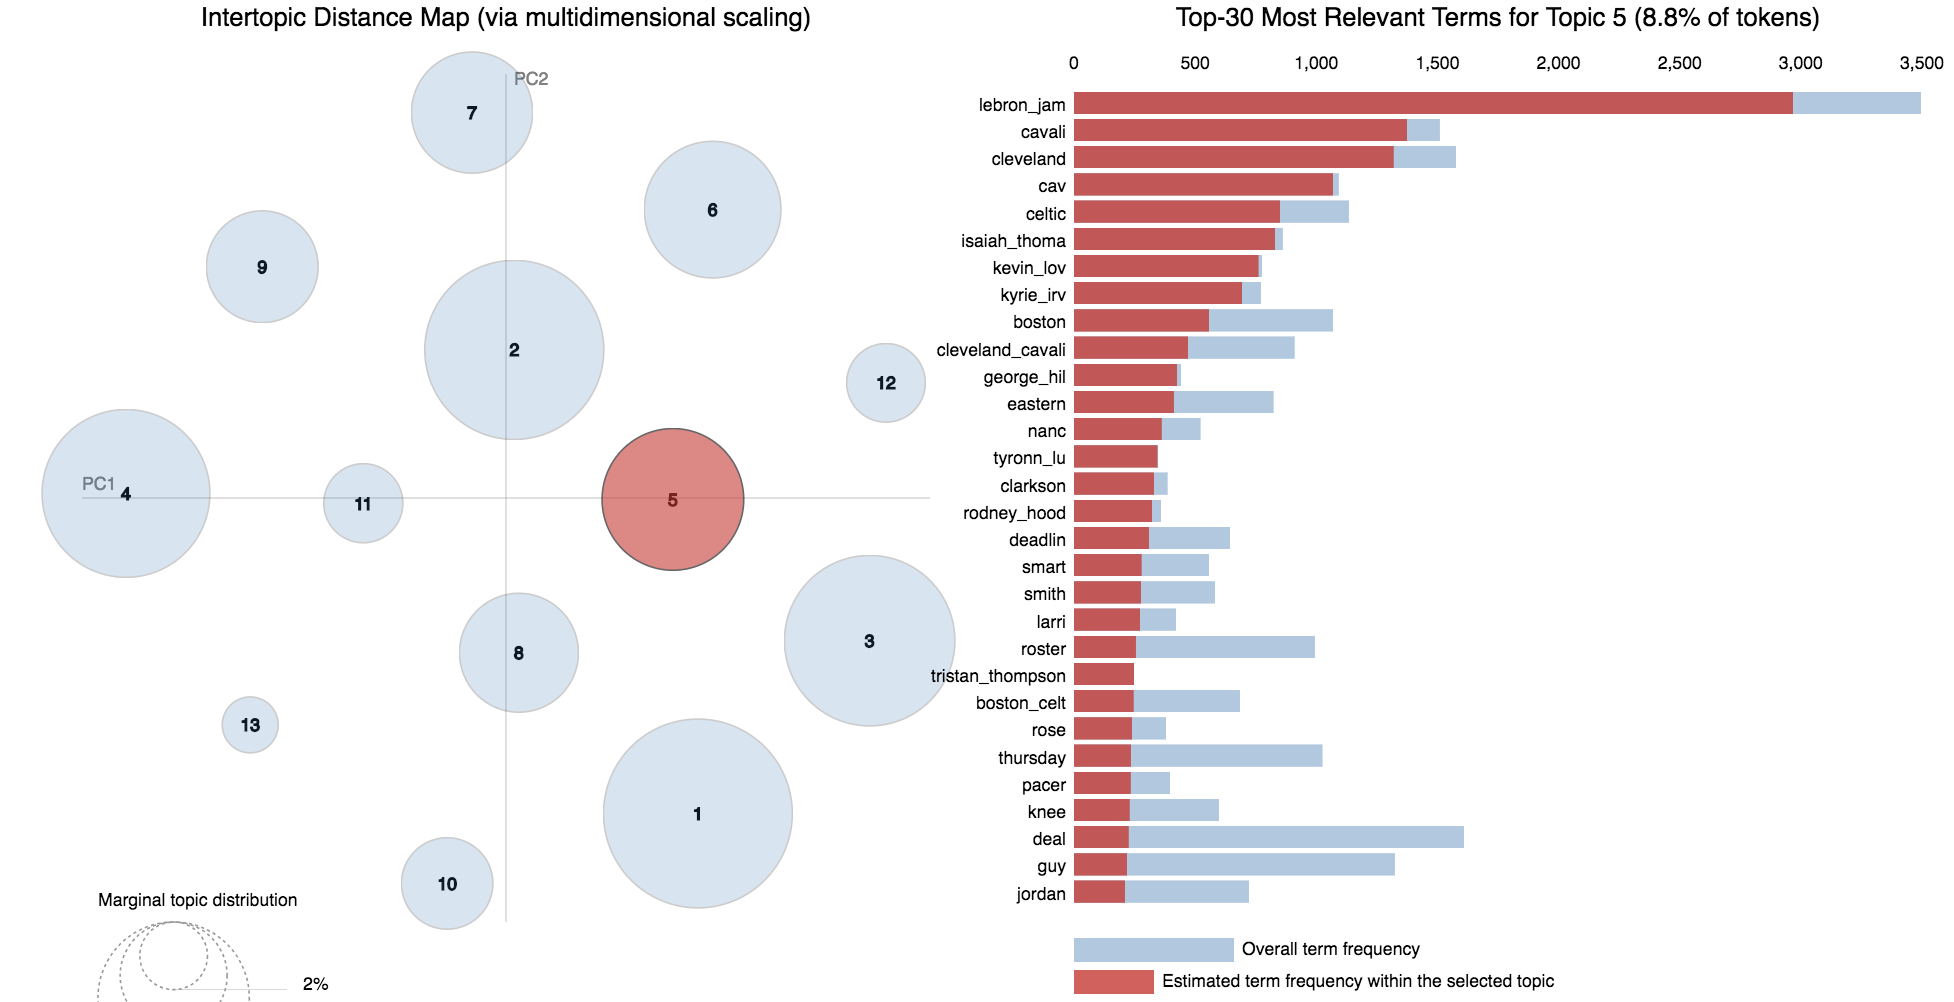
\includegraphics[width=470pt]{5.png} 

In fact, if you hover over the term \textit{lebron\_james}, you can see his primary topics. Topic 5 dominates as his primary topic. 

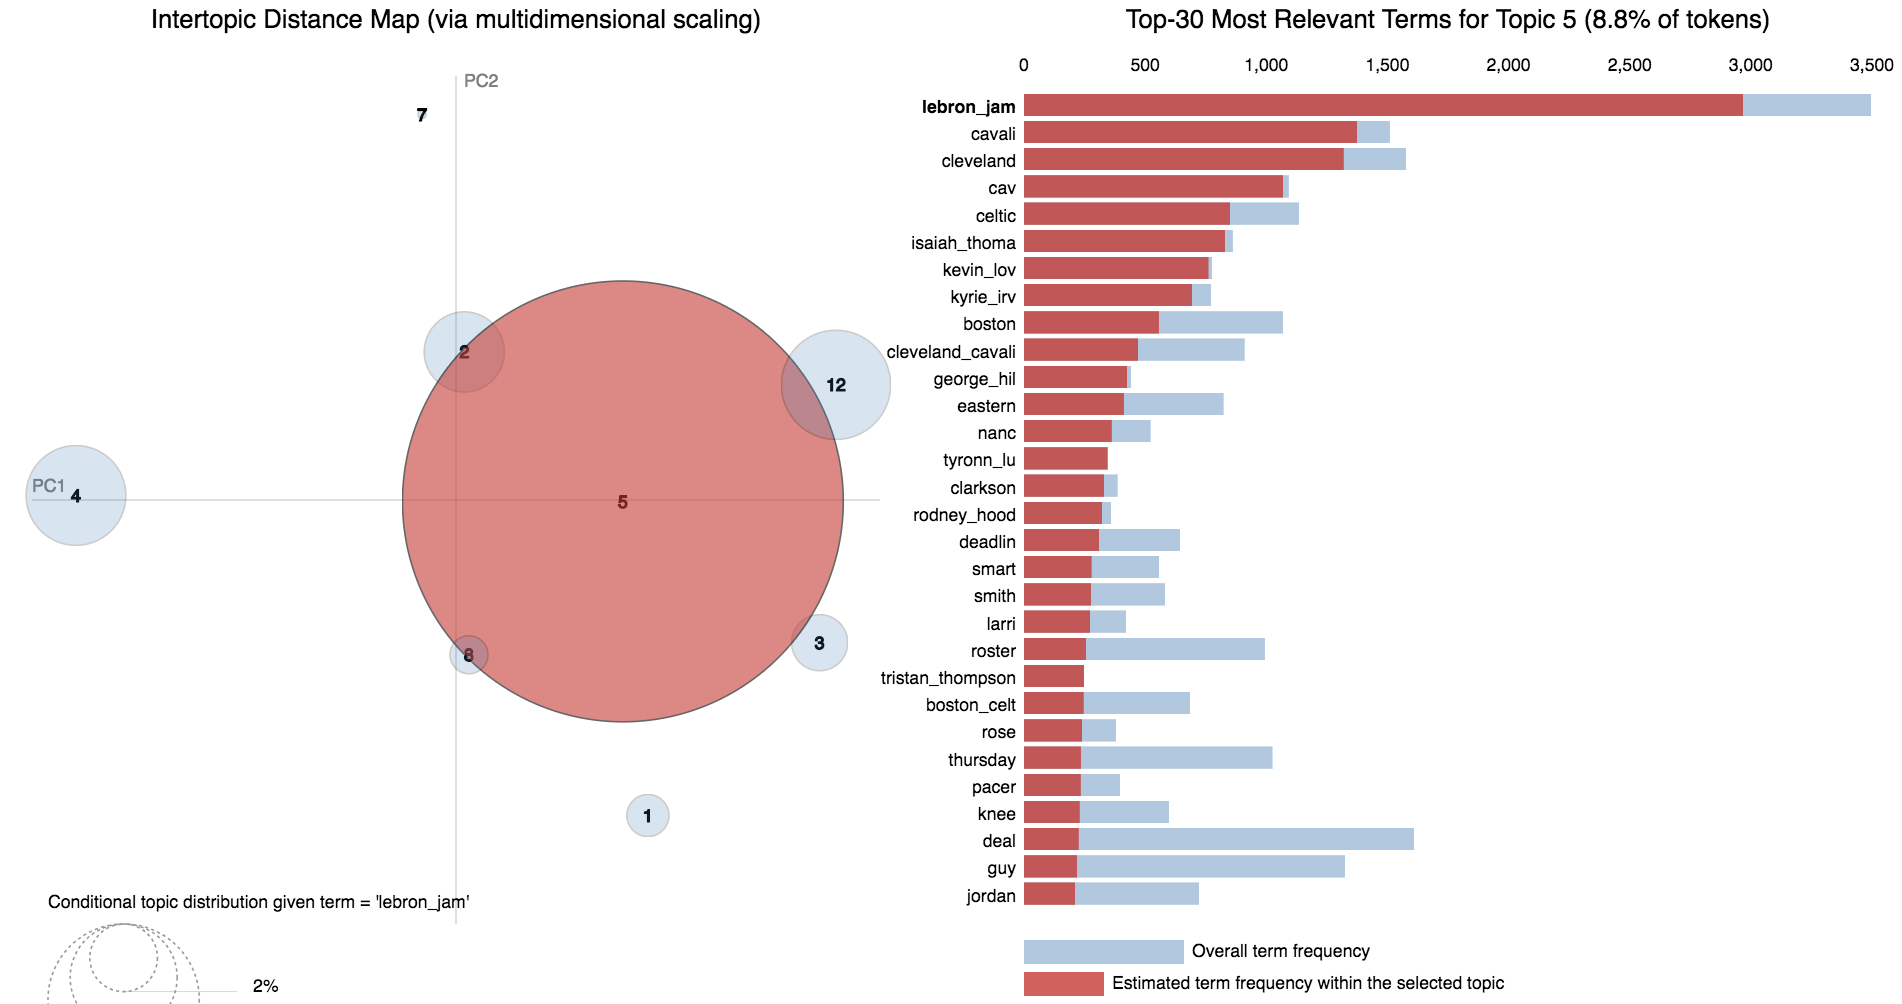
\includegraphics[width=470pt]{6_lebron.png} 


Topic 6 collected the terms pertaining to the NCAA March Madness college basketball tournament, which pushes aside the NBA in popularity for a brief month as the college kids take center stage. Michigan played Villanova for the championship this year. \\
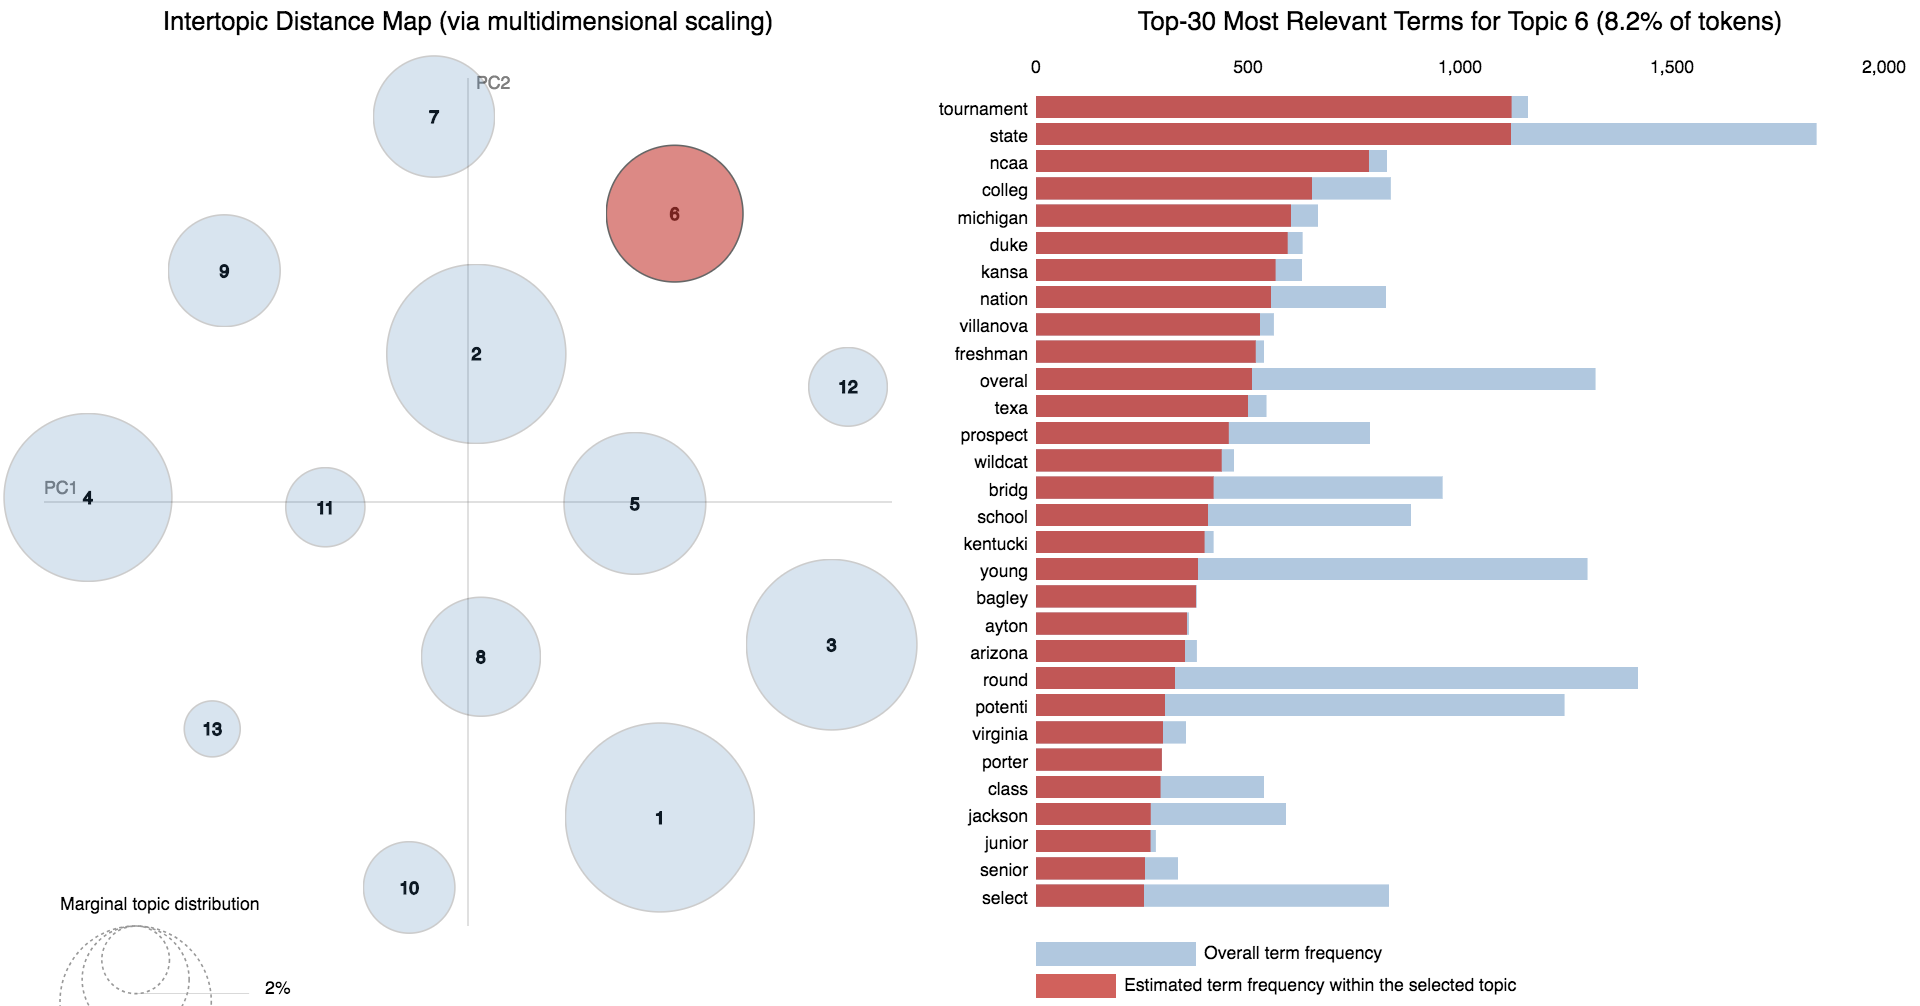
\includegraphics[width=470pt]{6.png} \\

Topic 7 seems to be about the playoffs, seeding, and exciting first-round matchups.  \\
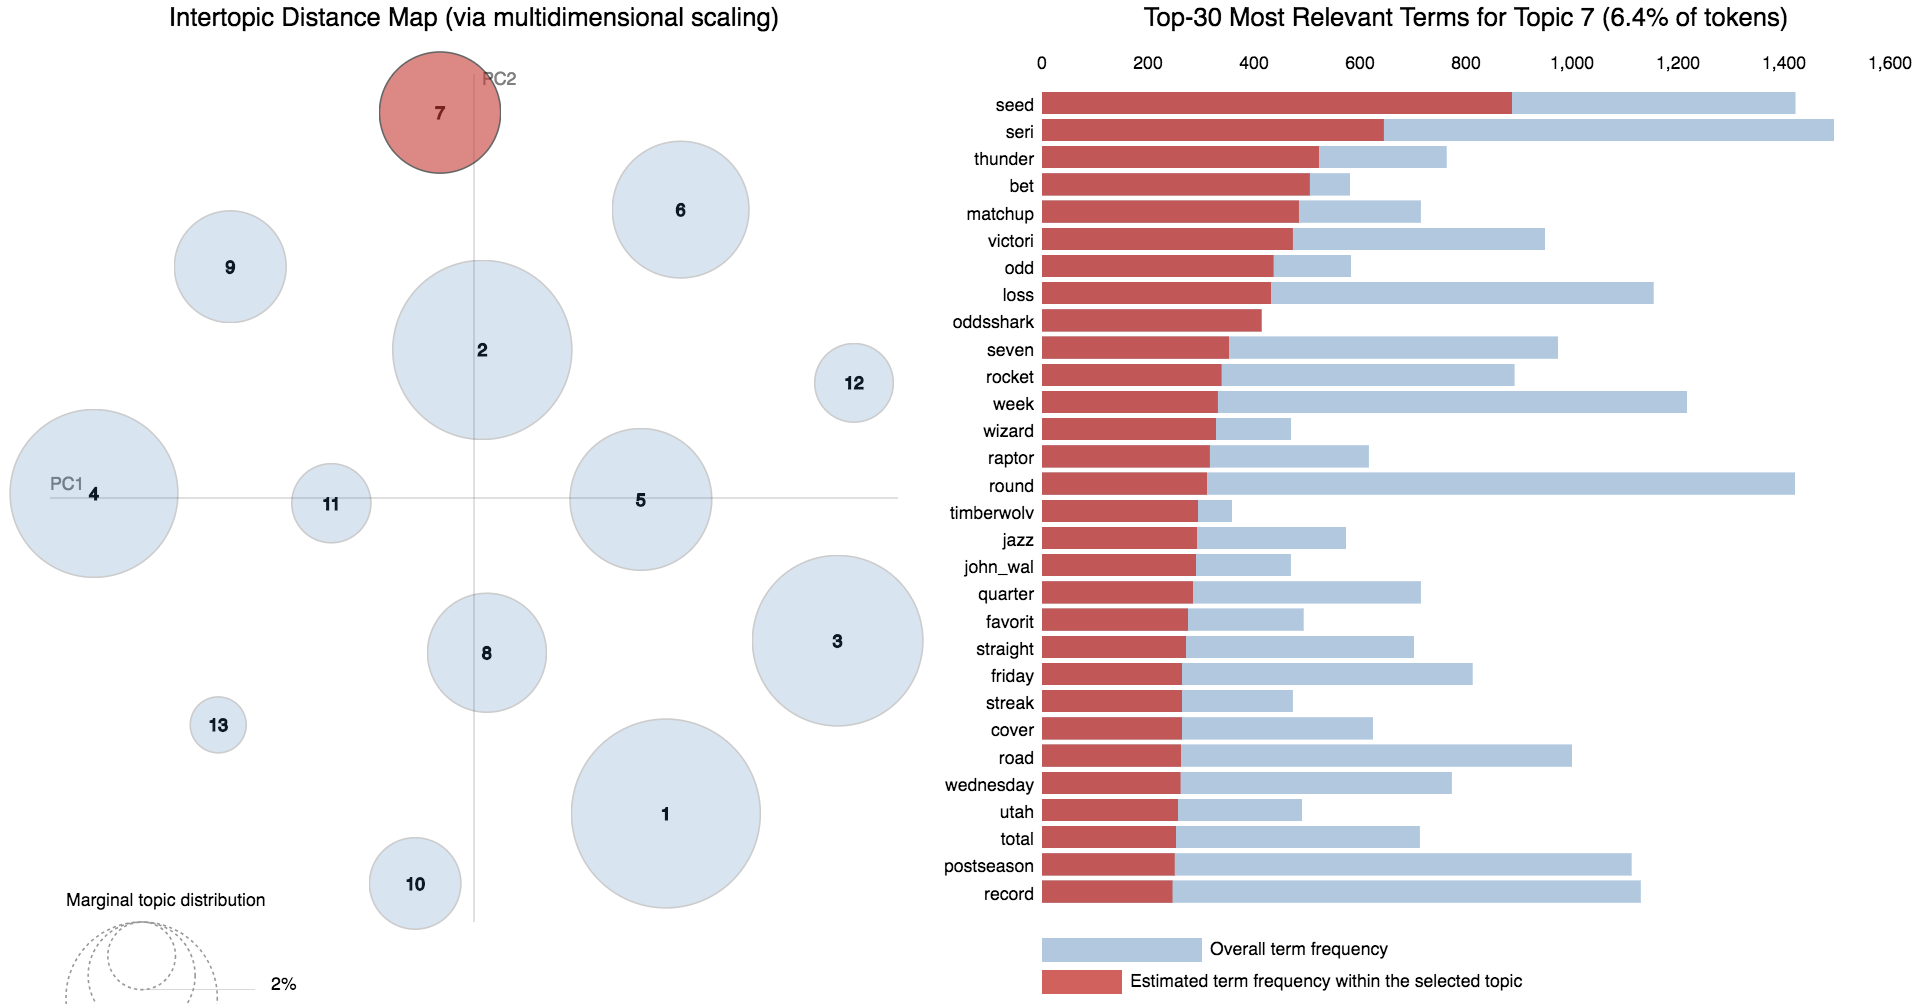
\includegraphics[width=470pt]{7.png} \\

Topic 13 is actually about soccer!  The NewsAPI must have returned a handful of soccer-related articles with the basketball ones, and our LDA model discovered that. \\
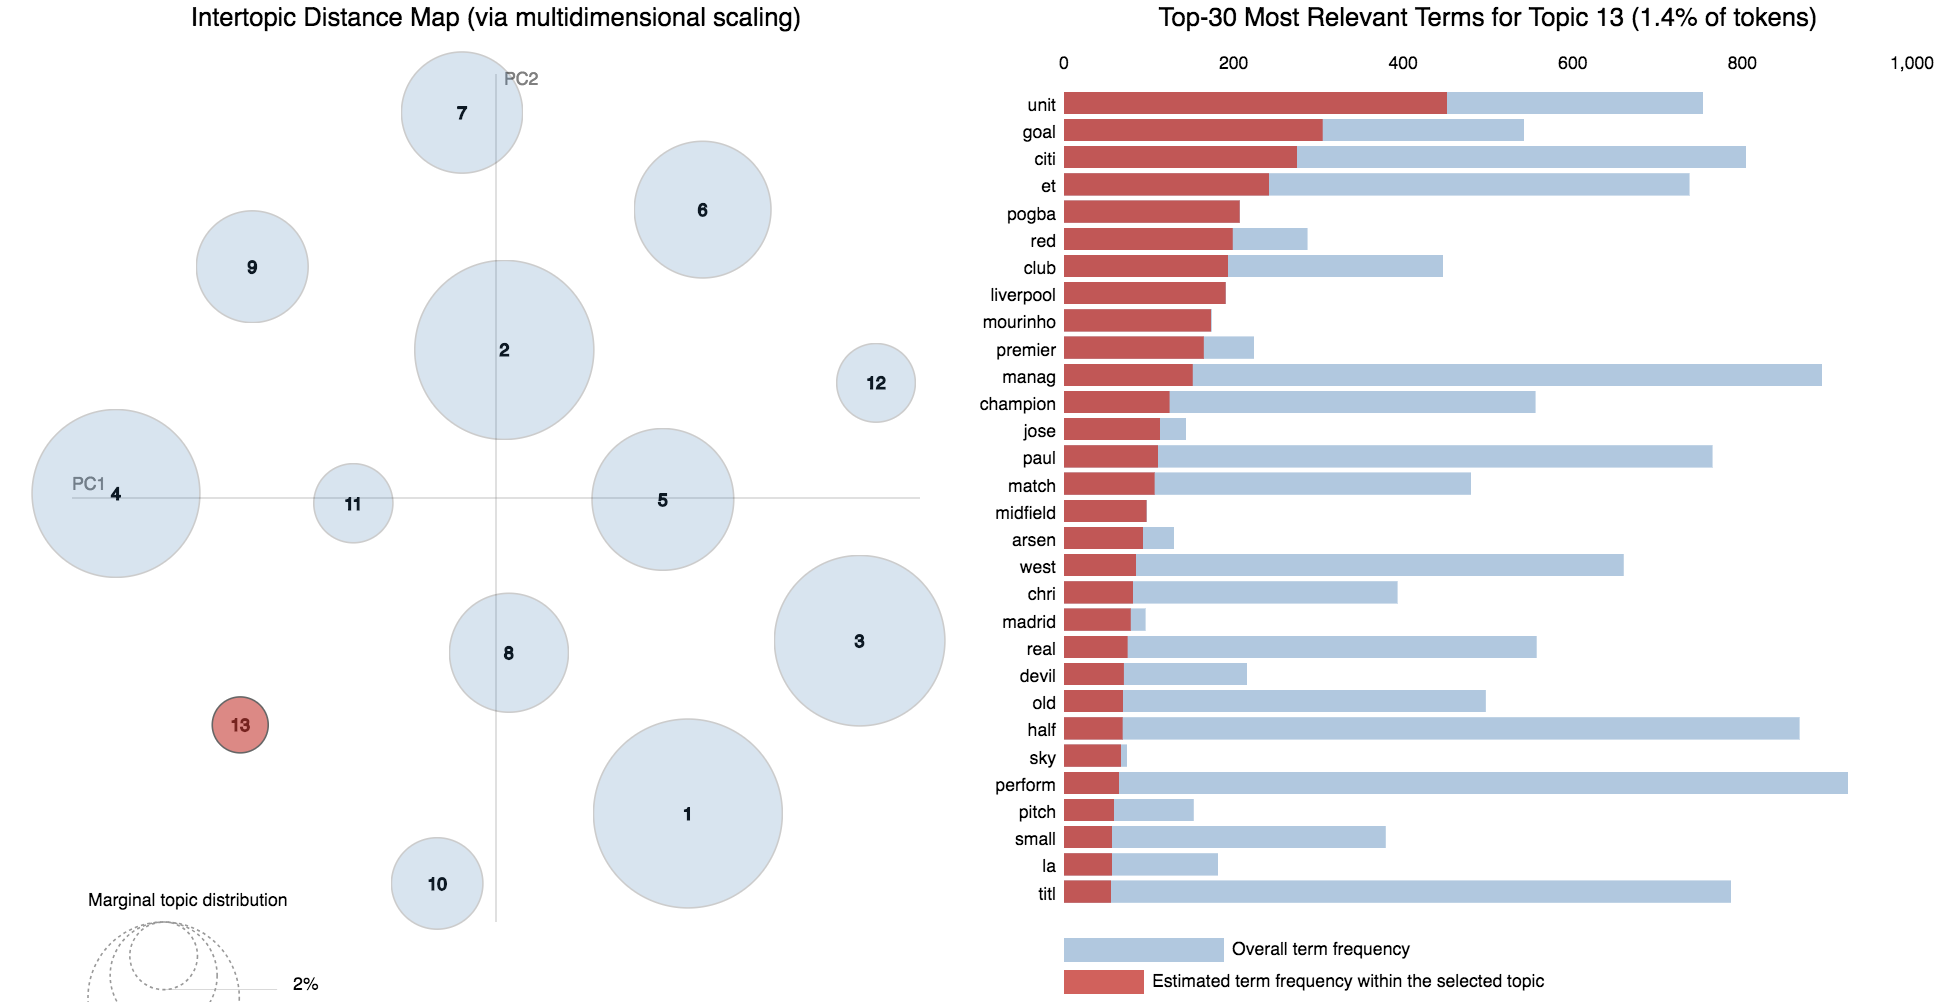
\includegraphics[width=470pt]{13.png} \\

We have left the other topics in the appendix for brevity.

\section{Producing a Recommendation: An Example}
Let us see our recommender system in action.  We took a new article from May 13, 2018, entitled \textit{Keith Pompey on 76ers' Pursuit of Lebron James: Prepared to Do Whatever It Takes}, and expressed it as a distribution over the 13 topics using our trained LDA model.  Here is the distribution over topics.  We've labeled each topic according to what we think it primarily represents (as specified above and in the appendix). Not suprsingly, this article is mostly about free agency and trades. Also, notice that the topic of the 76ers is prominent. 

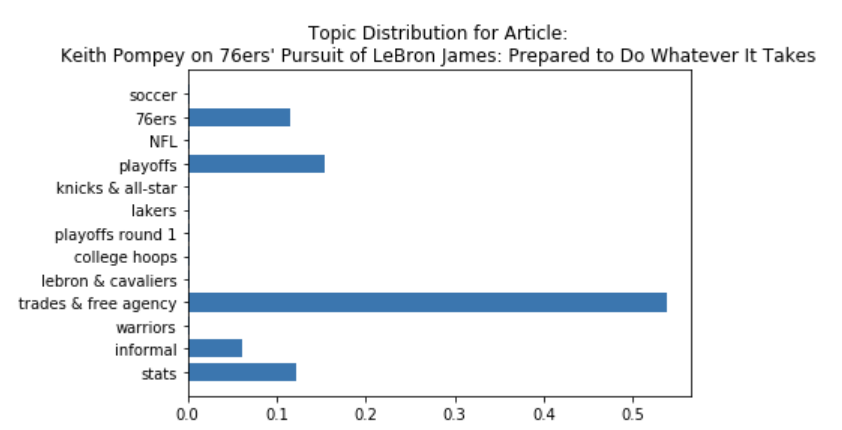
\includegraphics[width=300pt]{newarttopics.png}\\

Then, we found the nearest article to it using L2 norm, from all articles in the Bleacher Report corpus expressed in terms of their topic mixtures. Here's are the top 5 recommendations: \\
 
 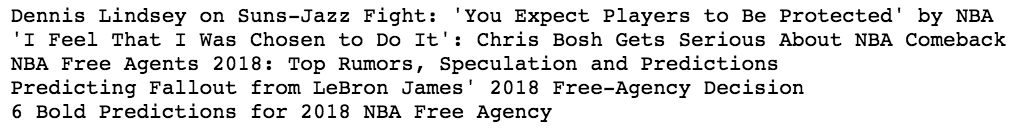
\includegraphics{preds.png}\\
 
 While some articles feel like they are not relevant (notably the first two), notice that the other three recommendations are on-point in discussing Lebron James' upcoming free agency decisions. 

\section{Discussion}
Most of the world's data is in the form of unstructured natural language, and using Natural Language Processings provides an analytics edge in many domains, not the least of which is online advertising.  It is no surprise that NLP is one of the hottest fields in research right now.  In this project we learned a lot about NLP, from data cleaning and data scraping to building topic models on a corpus of articles.  We learned a lot about three common ways of embedding documents in a vector space, and then took a deep dive into training and visualizing one of them, Topic Modeling with Latent Dirichlet Allocation. The vector-space article embedding was motivated by a desire to cluster articles to produce quality recommendations.  If hired by Bleacher Report, our first step would be to do a live test of our LDA-based recommender system.  

\section{Appendix}
\subsection{Initial Experiment to Find Most Promising Model}
\subsubsection{Word2vec}
Word2vec is a modeling approach that aims to embed words as vectors by considering their context in a corpus.  In a successful model, words that share common contexts correspond to vectors in close proximity in the space.  In our case, we with to embed \textit{articles}, not words,  so the approach we tested was to \textit{average the word embeddings in the title of the article}. 
%\subsubsection{Word2vec Pre-processing}
Word2vec training requires a set of sentences, not documents, so we began a different data-processing pipeline just for this model, starting from the scraped documents. In addition, we left in all of the words, as opposed to removing them as in the other models. The reason for this is that word2vec infers dependency information between words, and removing stop words would remove that linkage information.
%\subsubsection{Word2vec Training}
The number of word2vec dimensions is a hyperparameter that depends on the application. Most literature recommends a value of 100, and this produced very reasonable results in our case.

The closest vectors to lebron\_james are his (all-star) teammates, his hometown, his team name, and his trash-talking nemesis and other all-star rivals. \\
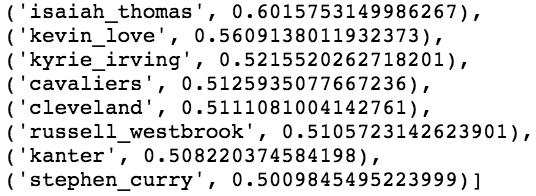
\includegraphics[width=200pt]{james_word2vec.png} 

The model correctly separates teams from the Eastern Conference from teams in the Western Conference, which you would expect from a Bleacher Report corpus with many articles about each conference separately. The model also places team mates in close proximity and can differentiate between teammates and non teammates. \\
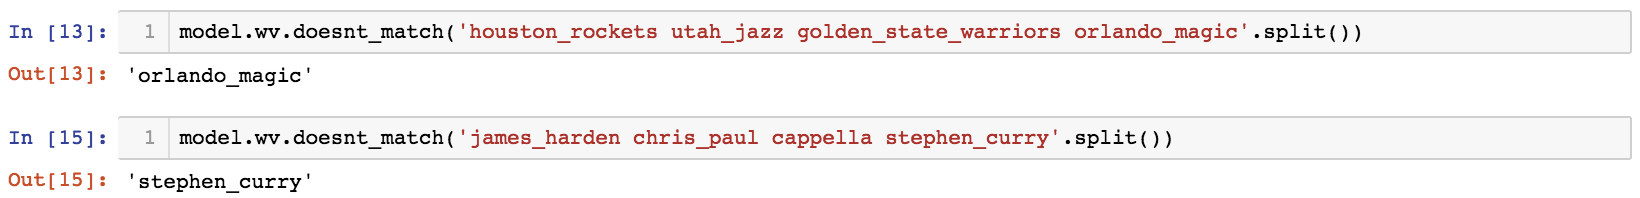
\includegraphics[width=450pt]{word2vec_diffs.png} 

\subsubsection{Non-Negative Matrix Factorization}
NMF is a topic modeling approach blah blah blah
(CYRILLE INSERT INFO HERE)

\subsubsection{Experimental Results: LDA Wins}
we acknowledge that this isn't rigorous blah blah blah
(WE NEED TO FILL IN THIS SECTION WITH OUR EXPERIMENT DETAILS)

%%%%%%%%%%%%%%%%%%%%%%%%%%%%%%%%%%%%%%%%%%%%%%%%%%%%%

Topic 8 seems to capture the multiple stories around the Los Angeles Lakers this season, always a popular NBA team. 

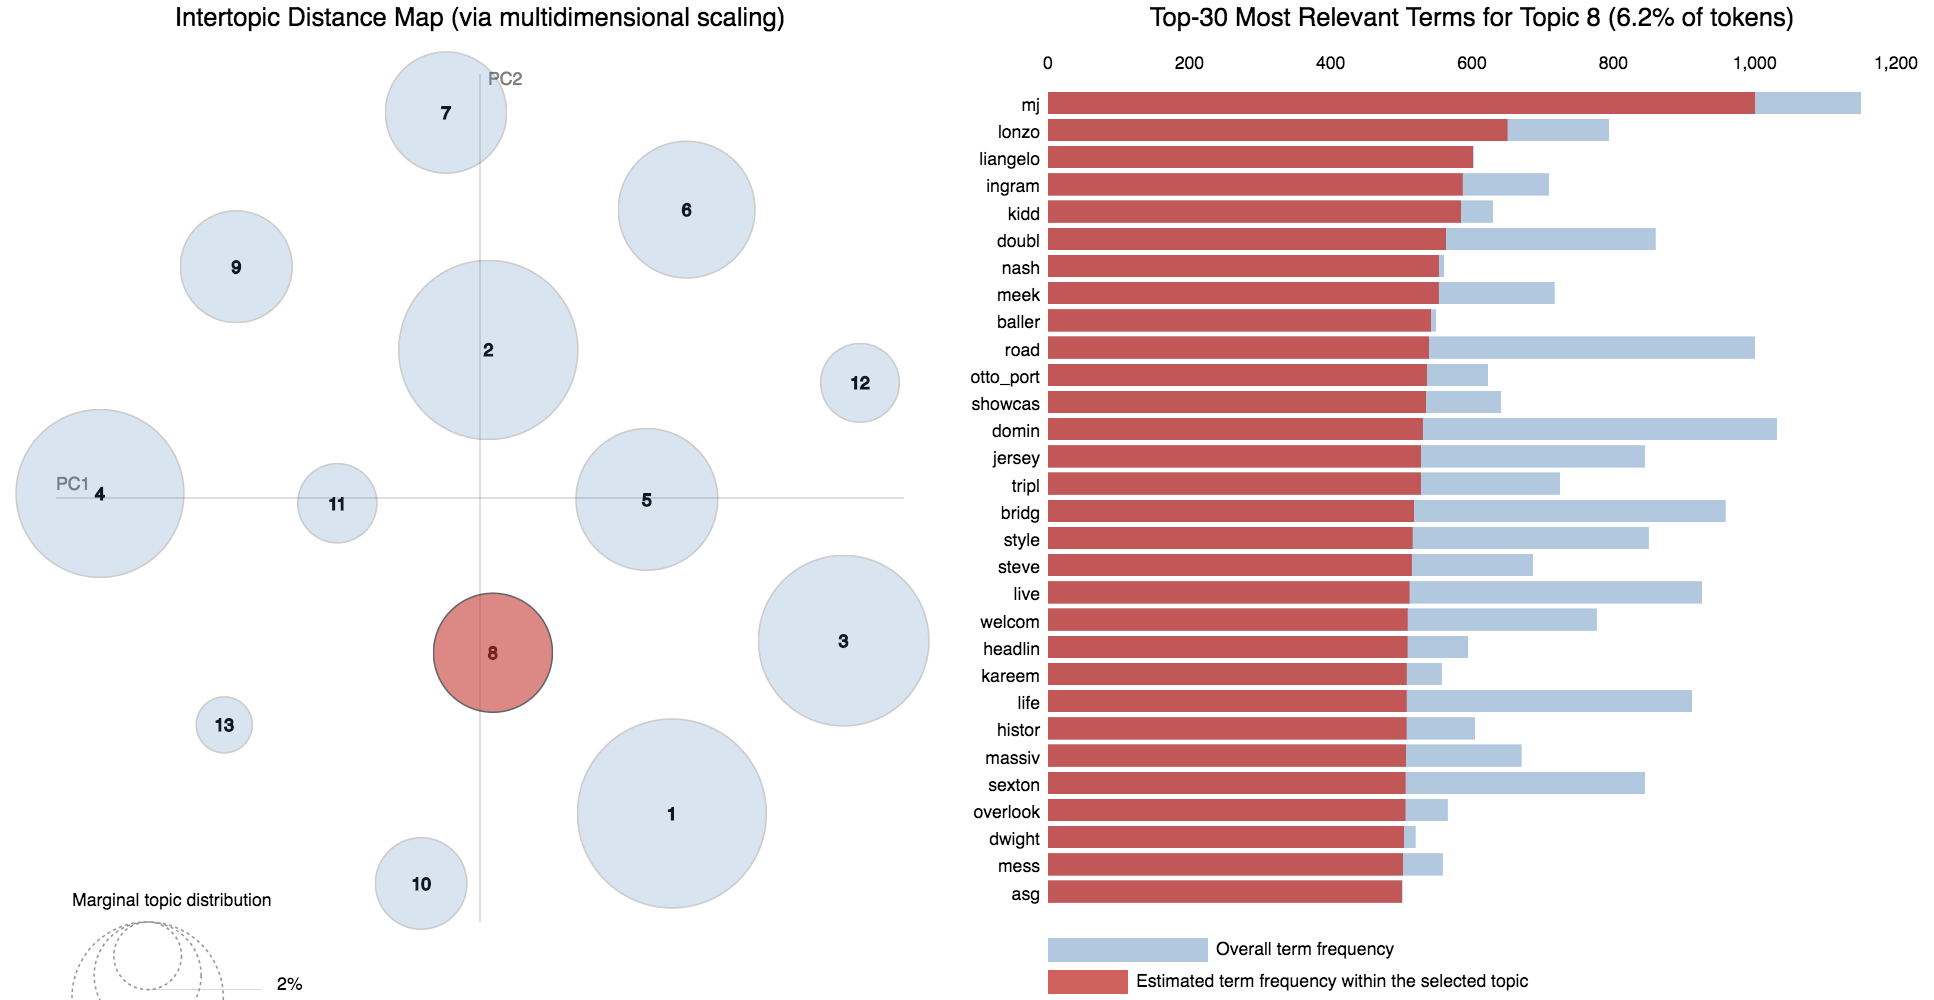
\includegraphics[width=470pt]{8.png} 

Topic 9 seems to merge two distinct topics, in our opinion - the all-star game and the New York Knicks. 

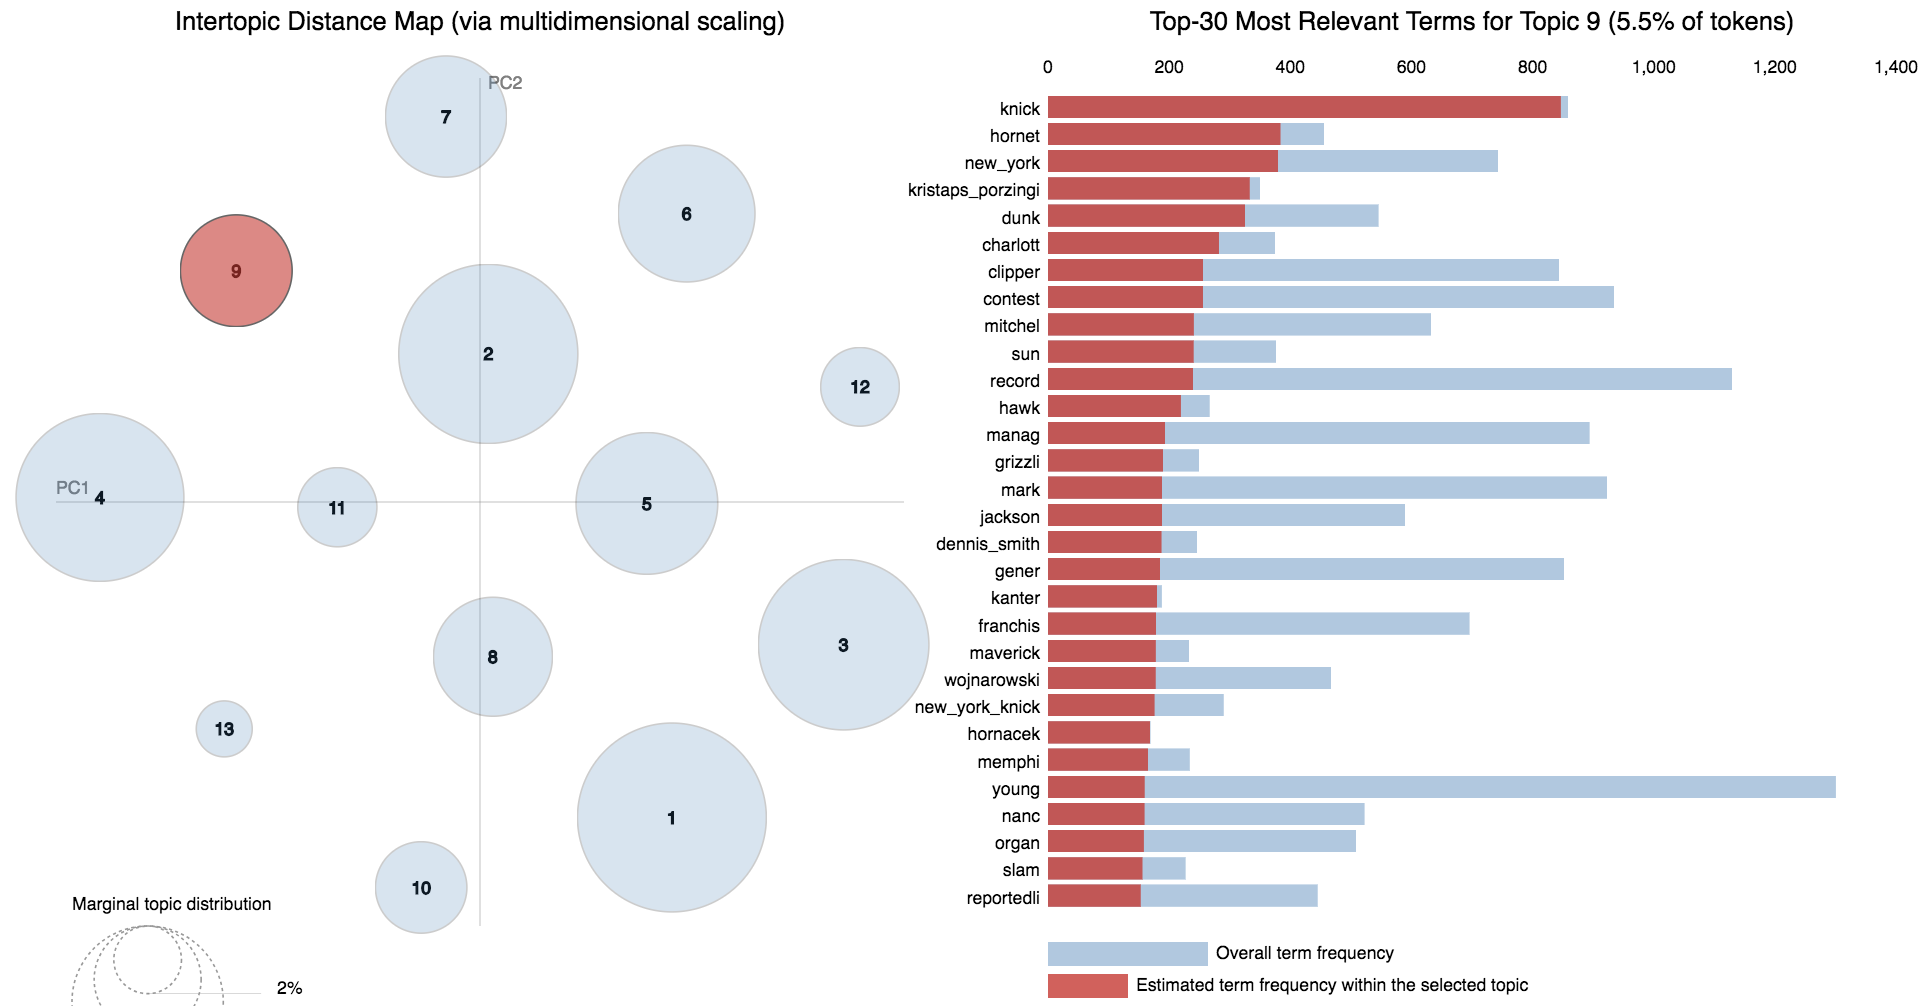
\includegraphics[width=470pt]{9.png} 

Topic 10 is about the playoffs, and includes the most notable postseason teams. 

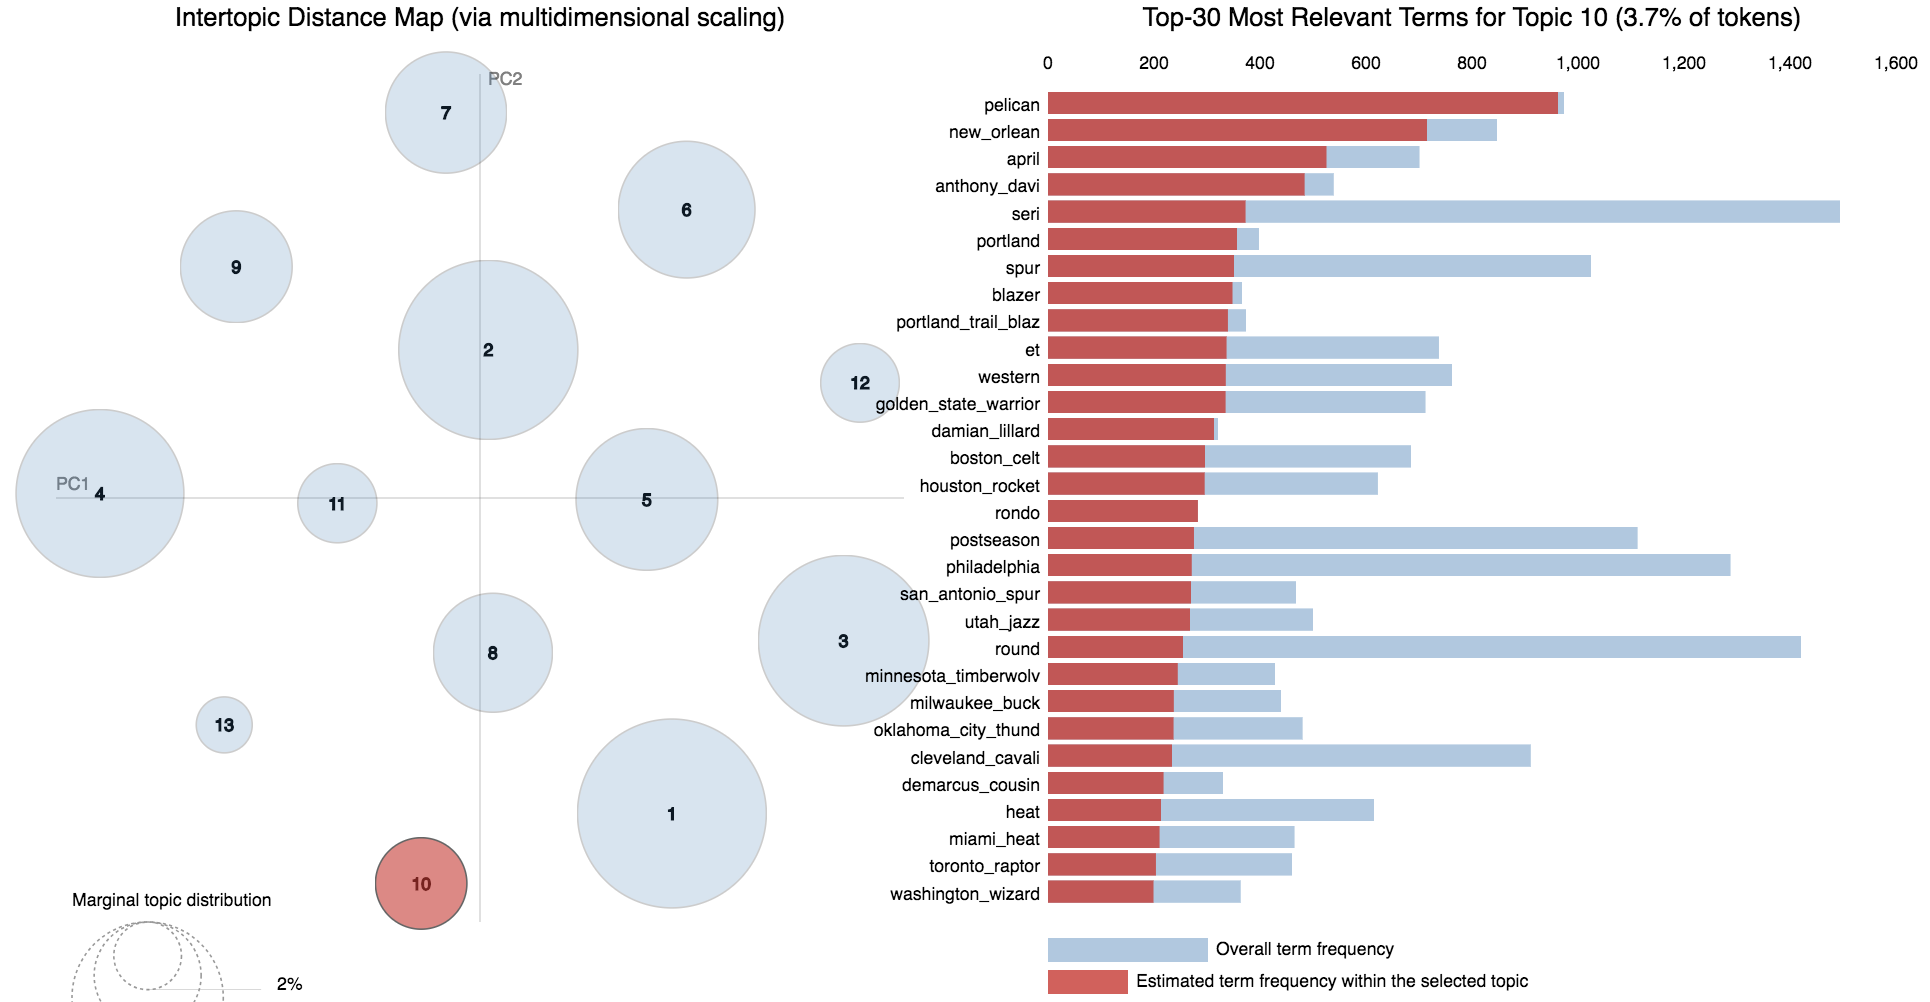
\includegraphics[width=470pt]{10.png} 

Topic 11 is actually about the National Football League!  The NewsAPI must have returned a handful of football related articles with the basketball ones, and our LDA model discovered that. 

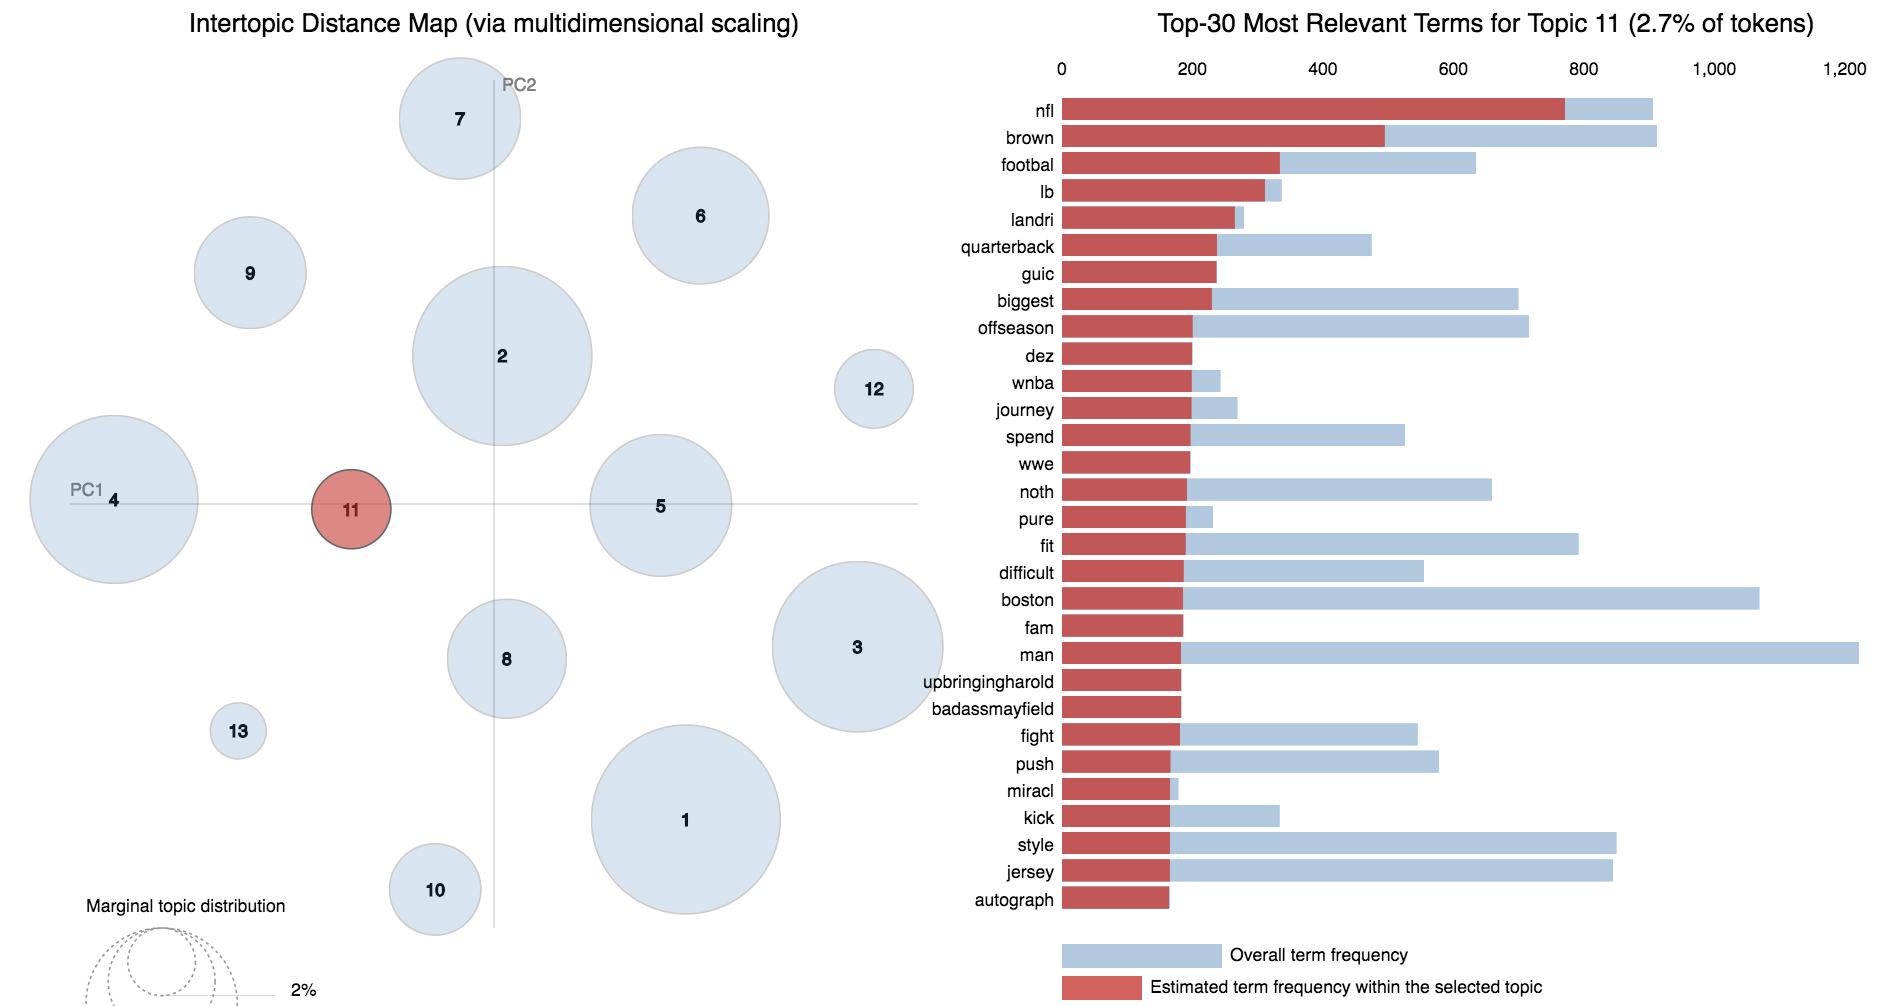
\includegraphics[width=470pt]{11.png} 

Topic 12 seems to be about the Philadelphia 76ers and their rivalry with the Miami Heat this season. The 76ers have been one of this seasons biggest sub-stories because they have two budding young superstars and are seeking to land Lebron James during free agency this summer.

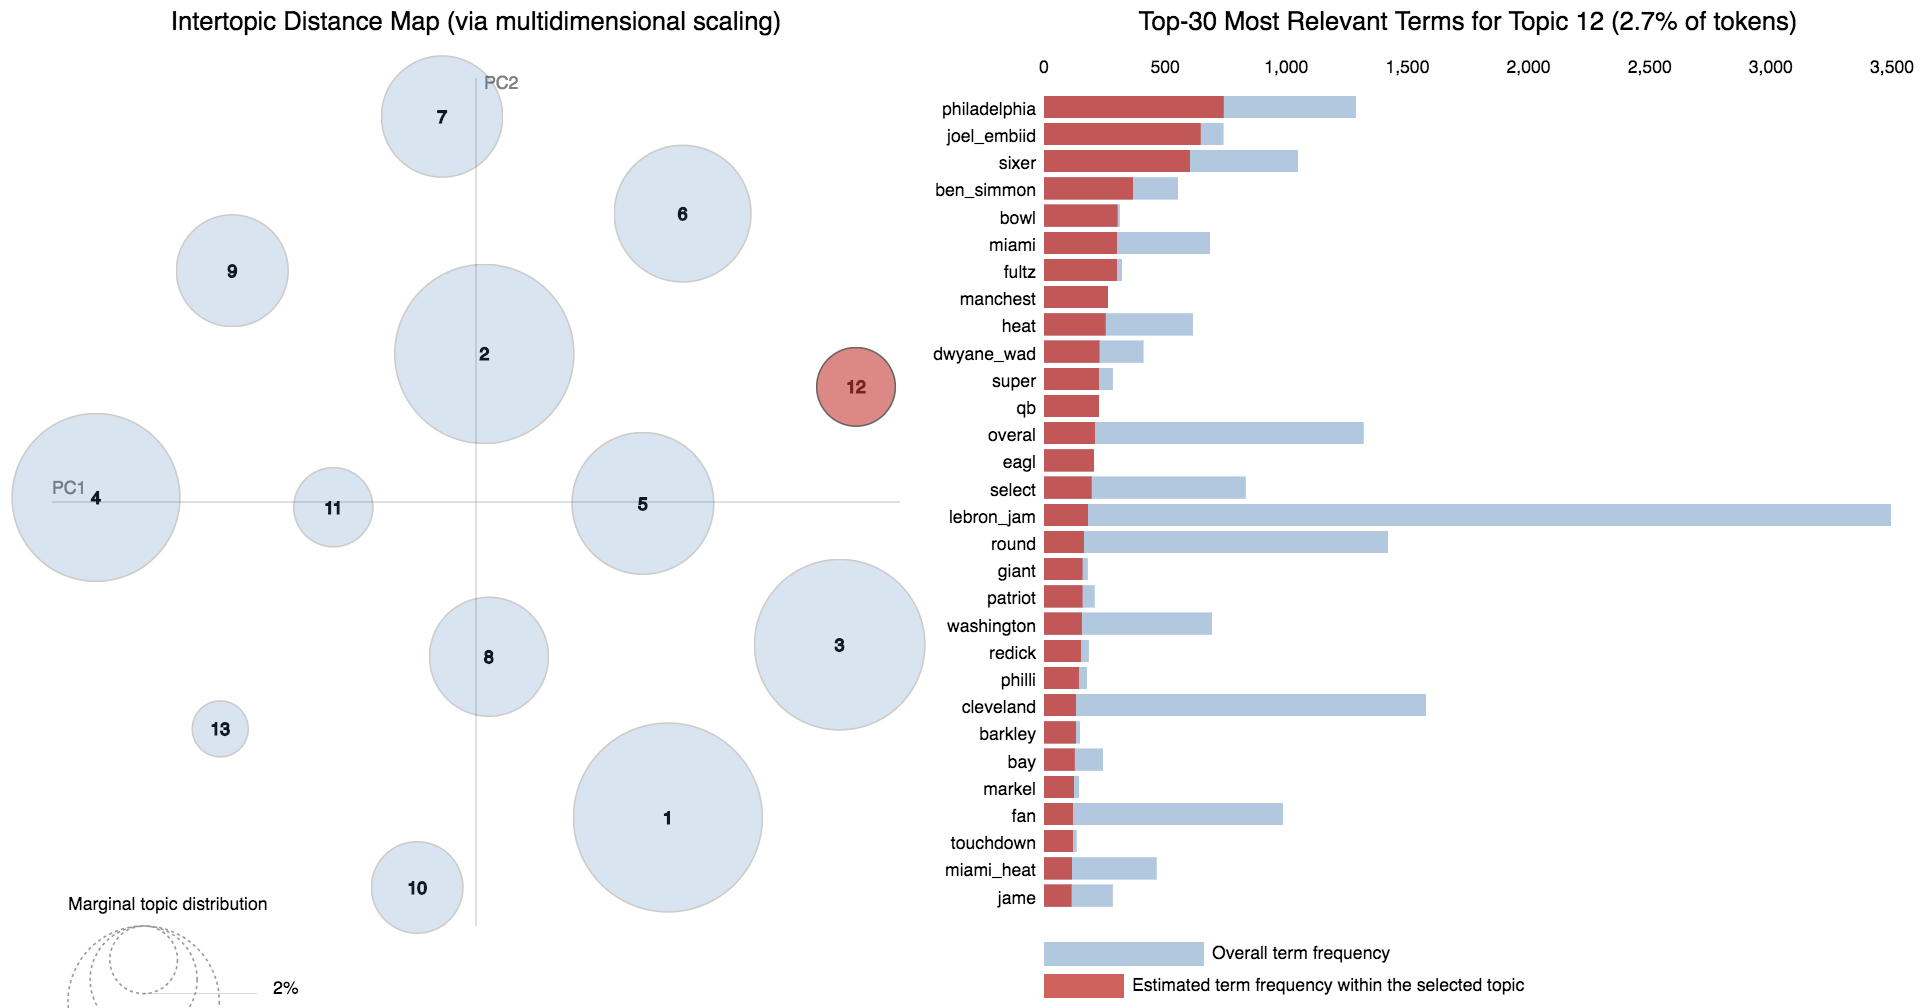
\includegraphics[width=470pt]{12.png} 

Topic 2, located in the middle of the topic clusters, seems to capture informal language. 

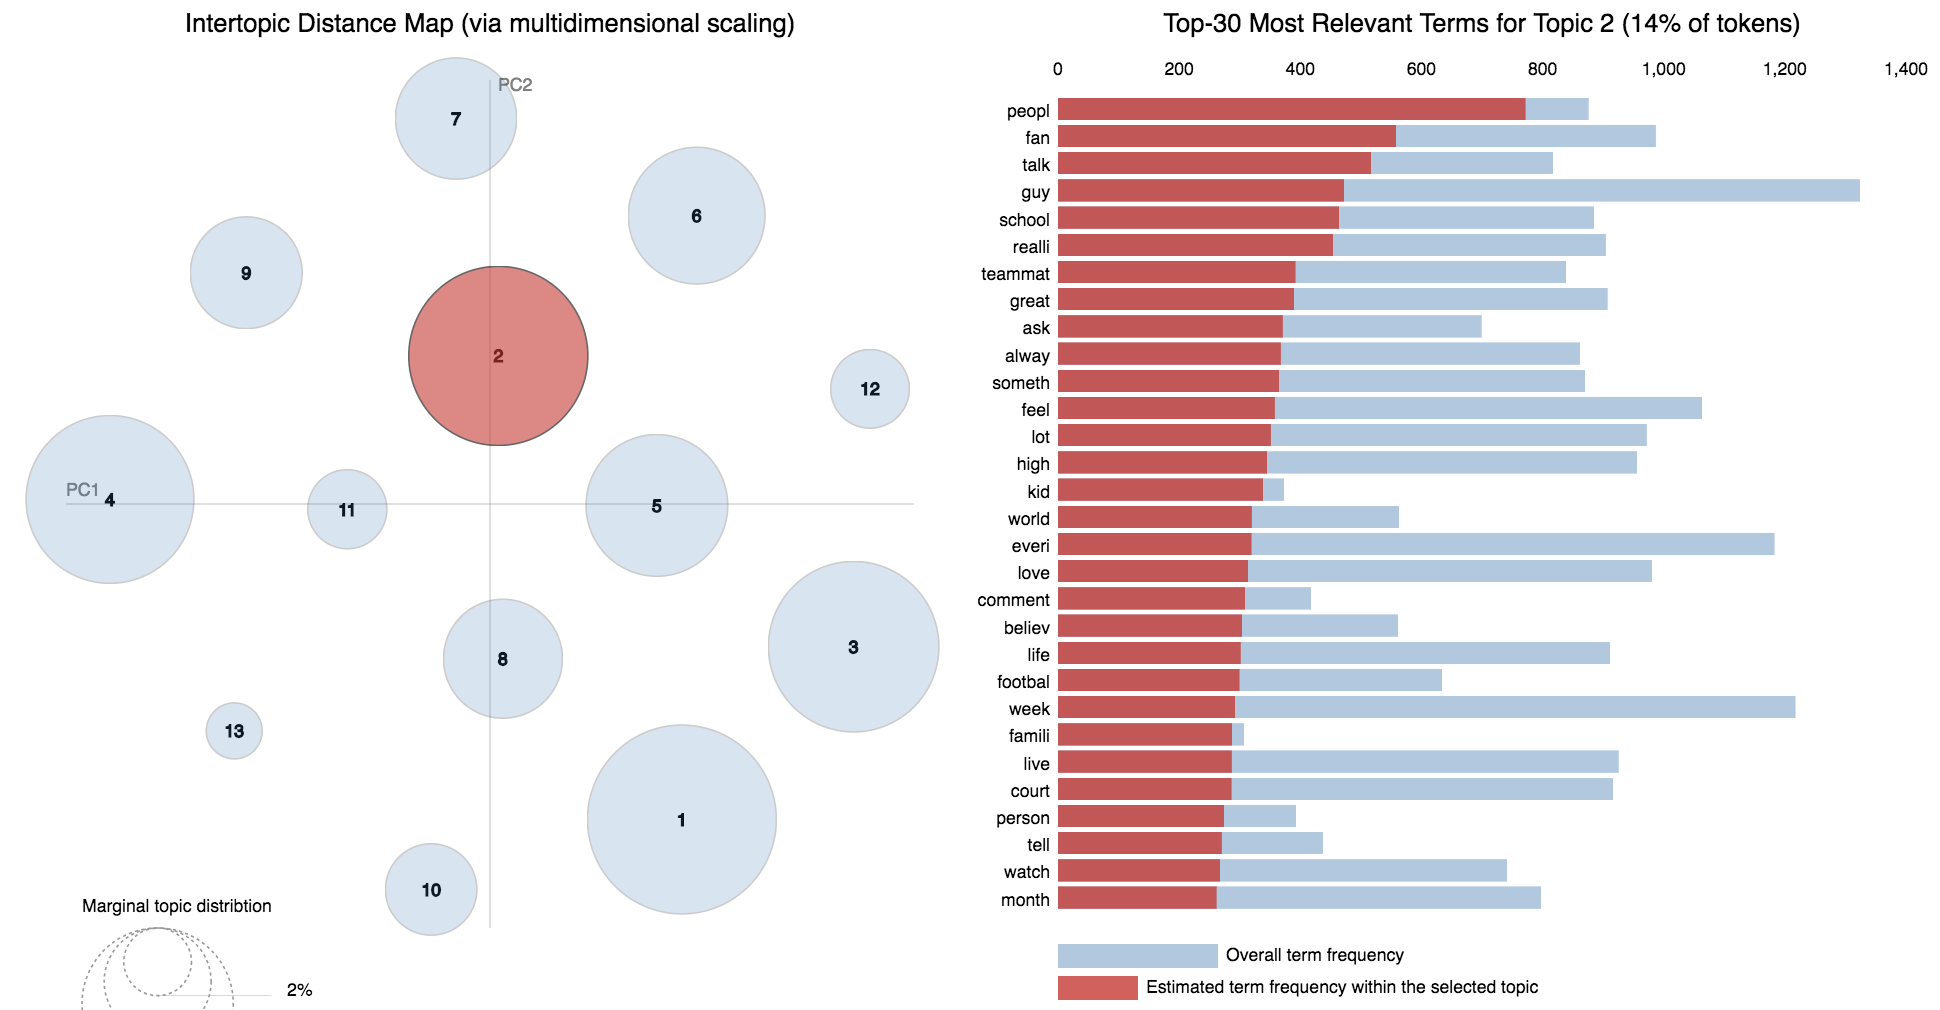
\includegraphics[width=470pt]{2.png} 

\end{document}